\documentclass[11pt, a4paper]{article}

\usepackage{geometry}
\geometry{a4paper, margin=2.5cm}
\usepackage[utf8]{inputenc}
\usepackage[T1]{fontenc}
\usepackage{lmodern}
\usepackage[spanish,es-tabla]{babel}
\usepackage{graphicx}
\usepackage{booktabs}
\usepackage{tabularx}
\usepackage{setspace}
\usepackage{float}
\usepackage{caption}

\captionsetup[figure]{name=Fig., labelsep=space}

\addto\captionsspanish{
  \renewcommand{\contentsname}{\hfill ÍNDICE \hfill}
}

\usepackage[colorlinks=true, linkcolor=black, urlcolor=blue, citecolor=black]{hyperref}

\begin{document}

\begin{titlepage}
    \centering
    
\includegraphics[width=0.4\textwidth]{logo.png}\\[1cm]
    
    {\Huge \textbf{Tecnológico\\de Monterrey}}\\[1cm]
    {\Large \textbf{INSTITUTO TECNOLÓGICO Y DE ESTUDIOS SUPERIORES DE MONTERREY}}\\[0.5cm]
    {\Large CAMPUS PUEBLA}\\[0.5cm]
    {\large Departamento de Ingeniería Mecatrónica}\\[2cm]
    
    {\Huge \textbf{Documentación}}\\[0.5cm]
    {\Huge \textbf{AMR TEC 1}}\\[2.5cm]
    
    \begin{flushleft}
    \textbf{Documentación elaborada por:}\\
    De La Trinidad Rendón Julio Sebastián \hfill | A01732896\\
    Huerta Sedeño Tomas \hfill | A01329035\\
    Martínez Ayala Miguel Alejandro \hfill | A01734990\\
    Reyes Brito Ali Abigail \hfill | A01730642\\
    González Rodríguez Pedro Samuel \hfill | A01732105\\[1cm]
    
    \textbf{Docentes:}\\
    Balbuena Palma José Ángel\\
    Flores Quintero Roberto Rafael\\
    Medina Pozos José Manuel\\
    Mora Salinas Roberto Julián\\
    Ramírez Mendoza Arturo\\
    Reyes Avendaño Jorge Antonio\\
    Rojas Carreón José Jorge\\
    Varela Soriano Julio\\
    \end{flushleft}
    
    \vfill
    {\large H. Puebla de Zaragoza, Pue., a 23 de febrero del 2023}
\end{titlepage}

\newpage
\tableofcontents
\newpage

\section{Especificaciones}
\label{sec:especificaciones}

\subsection*{Dimensiones}
A continuación, se presenta una fotografía del AMR1, para tener una referencia de cómo se ve el vehículo (ver Fig. \ref{fig:amr1}).

\begin{figure}[H]
    \centering
    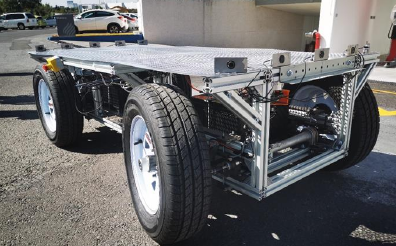
\includegraphics[width=0.8\textwidth]{figura1.png}
    \caption{Fotografía del AMR TEC 1.}
    \label{fig:amr1}
\end{figure}

\begin{itemize}
    \item \textbf{Largo:} 2.00 m
    \item \textbf{Ancho:} 1.08 m
    \item \textbf{Altura de chasis:} 0.435 m
    \item \textbf{Altura total:} 0.62 m
    \item \textbf{Peso:} 400 kg
\end{itemize}

\section{Descripción general}
\label{sec:descripcion_general}
El AMR TEC 1 (Autonomous Mobile Robot Tec 1), es un vehículo terrestre no tripulado con dirección tipo Ackerman que se pretende que sea autónomo. El objetivo principal de éste es que se utilice para el traslado de paquetes, materiales y otros objetos dentro del Tecnológico de Monterrey Campus Puebla.

Actualmente, la parte electrónica del vehículo está dividida en varios sistemas principales que lo dotan de la capacidad de moverse de una forma segura (se puede ver la ubicación de cada uno de ellos en la Fig. \ref{fig:vista_aerea}), cada uno de ellos tiene una función específica, y a continuación se describen de forma general.

\begin{figure}[H]
    \centering
    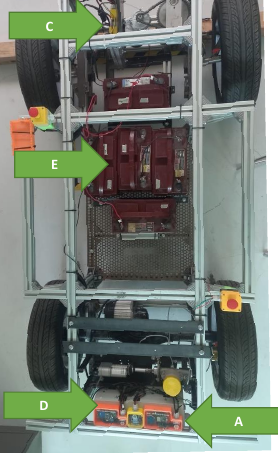
\includegraphics[width=0.6\textwidth]{figura2.png}
    \caption{Vista aérea del AMR1, con la localización de los sistemas principales.}
    \label{fig:vista_aerea}
\end{figure}

\subsection{Interprete CAN BT}
\label{subsec:gen_interprete}
Este sistema es el encargado de recibir los comandos, ya sea a través de Bluetooth o por medio de un control remoto, y de convertirlos a comandos CAN, que después mandará al resto de los sistemas del AMR. Éste hace uso de un ESP32, y aprovecha los dos núcleos que éste tiene para manejar de manera independiente la transmisión y la recepción de información. En la Fig. \ref{fig:vista_aerea}, se puede ver que el sistema se localiza en el punto A, en la parte trasera izquierda del vehículo, justo detrás de la bomba de frenos. Todo el sistema se describe de una forma más detallada en la sección \ref{sec:interprete_can}.

\subsection{Tren motriz}
\label{subsec:gen_tren_motriz}
Sistema encargado de generar el movimiento del vehículo. Hace uso de un motor trifásico y de un controlador UVW para generar la rotación de las llantas con una determinada velocidad y dirección, además, hace uso de un encoder para realizar el control de la velocidad del vehículo (está pendiente de implementar). Este sistema está implementado dentro del Tablero de control, en el lateral derecho del mismo (ver Fig. \ref{fig:tablero_control}), además, el motor trifásico se encuentra entre las llantas traseras del vehículo, alineado con los ejes de estas. Todo el sistema se describe de una forma más detallada en la sección \ref{sec:tren_motriz}.

\begin{figure}[H]
    \centering
    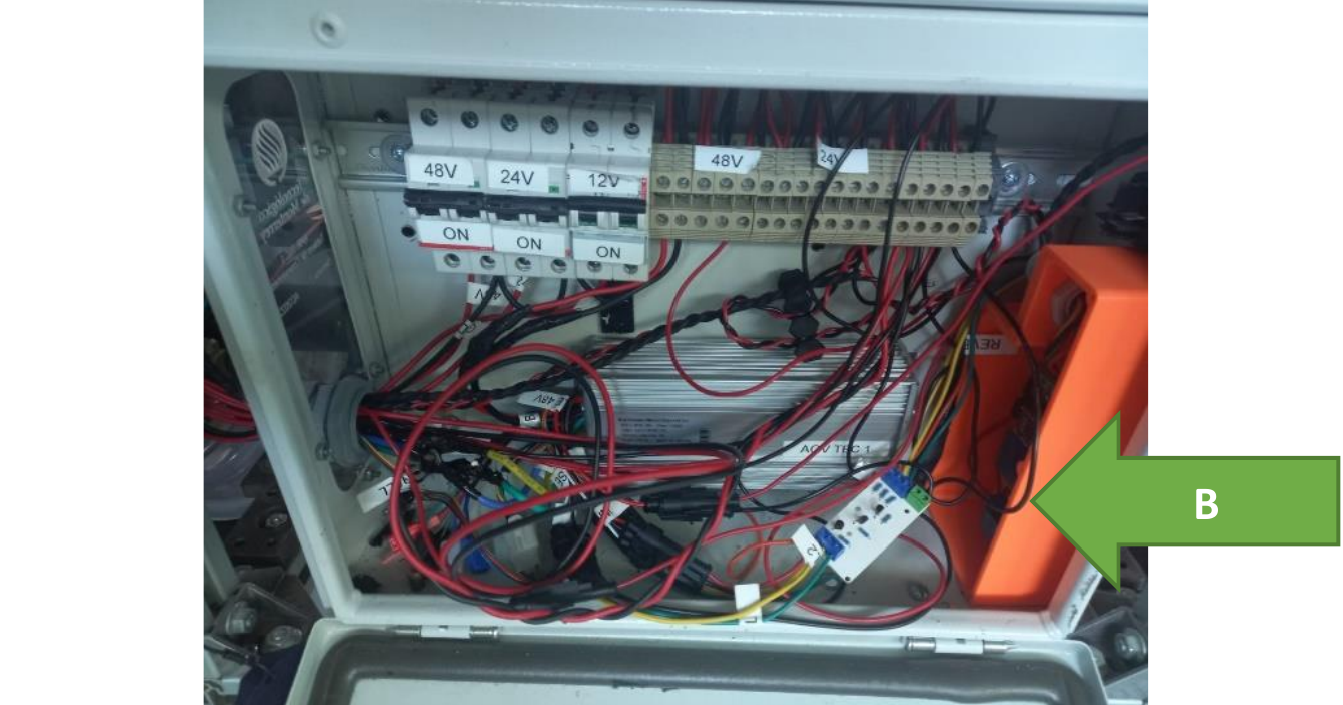
\includegraphics[width=0.7\textwidth]{figura3.png}
    \caption{Imagen del tablero de control, con la ubicación de las placas del tren motriz.}
    \label{fig:tablero_control}
\end{figure}

\subsection{Dirección}
\label{subsec:gen_direccion}
Sistema encargado de controlar la rotación de las llantas delanteras mediante una dirección tipo Ackerman. Se hace uso de un motor de corriente directa, el cual, mediante un sistema de engranajes transmite la rotación a la dirección. En la Fig. \ref{fig:tablero_control}, se puede ver que el sistema se localiza en el punto C, en la parte delantera del vehículo, en la parte derecha, se localiza el motor junto con el sistema de engranes, y en la izquierda toda la parte electrónica. Todo el sistema se describe de una forma más detallada en la sección \ref{sec:direccion}.

\subsection{Frenos}
\label{subsec:gen_frenos}
Sistema encargado de evitar que el vehículo se mueva. Éste hace uso de unos frenos de disco a los cuales les llega líquido mediante una bomba de líquido para frenos, la cual es activada por un actuador lineal. En la Fig. \ref{fig:vista_aerea}, se puede ver que el sistema se localiza en el punto D, en la parte trasera del vehículo; los frenos de discos están instalados en cada una de las llantas, la bomba está en la parte derecha y se puede identificar fácilmente por su tapa amarilla, el actuador está a la izquierda de la bomba, y todo el sistema electrónico está a la izquierda del módulo del intérprete. Además, dentro de este sistema también están incluidos los botones de paro de emergencia, los cuales se encuentran en los laterales del vehículo. Todo el sistema se describe de una forma más detallada en la sección \ref{sec:frenos}.

\subsection{Baterías}
\label{subsec:gen_baterias}
Sistema encargado de proporcionar la energía necesaria para alimentar a todo el vehículo. Actualmente consta de cinco baterías de 12 V, cuatro de ellas conectadas en serie para lograr un voltaje total de 48 V que alimentará al tren motriz, y la restante, conectada de forma independiente, para alimentar el resto de los sistemas. En la Fig. \ref{fig:vista_aerea}, se puede ver que el sistema se localiza en el punto E, en la parte de en medio del vehículo, un poco cargado hacia el frente. Todo el sistema se describe de una forma más detallada en la sección \ref{sec:baterias}.

\setcounter{section}{3}
\section{Secciones técnicas}
\label{sec:secciones_tecnicas}

\subsection{Interprete CAN BT}
\label{sec:interprete_can}

\begin{figure}[H]
    \centering
    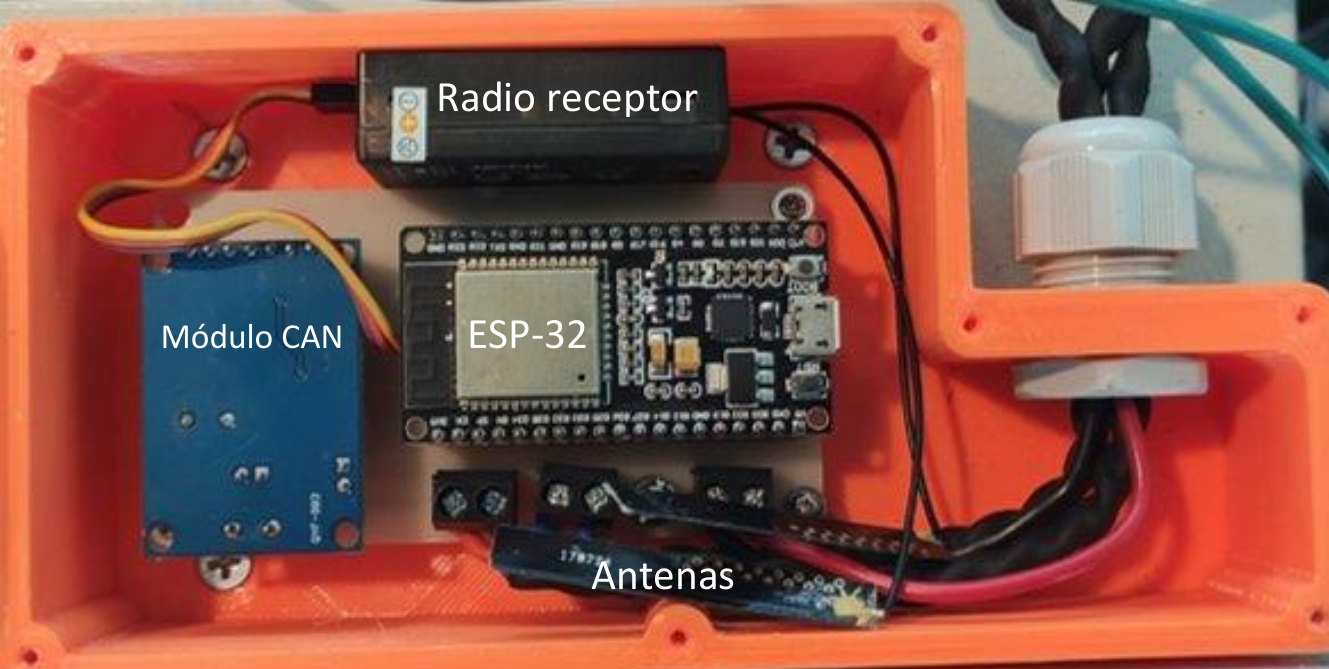
\includegraphics[width=0.7\textwidth]{figura4.png}
    \caption{Implementación del sistema de Interprete CAN BT.}
    \label{fig:impl_interprete}
\end{figure}

\begin{figure}[H]
    \centering
    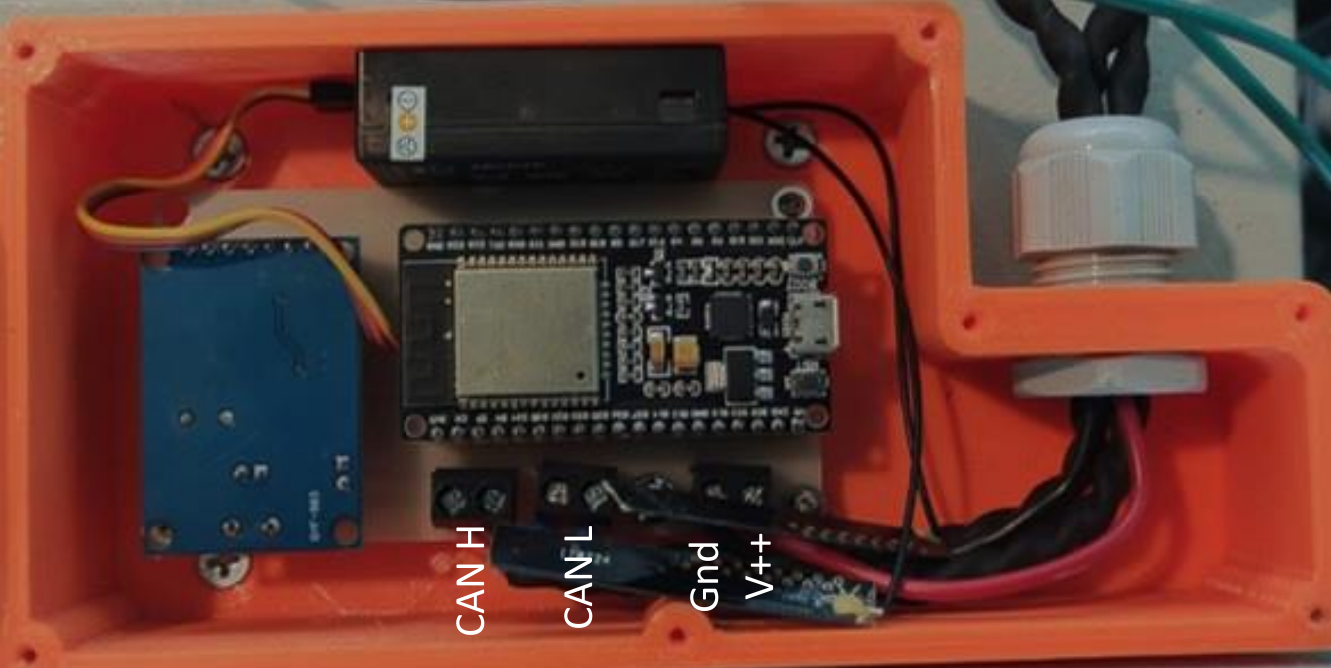
\includegraphics[width=0.7\textwidth]{figura5.png}
    \caption{Conexiones del Interprete CAN.}
    \label{fig:conexiones_interprete}
\end{figure}

El módulo de Interprete CAN BT es el encargado de recibir información, ya sea por medio de Bluetooth, o por medio de un control remoto, y mandarla en forma de comandos CAN al resto de los sistemas. Para el caso del Bluetooth, se usa la conexión de una computadora, y mediante la terminal, se ingresan literalmente los comandos CAN, mandando en primer lugar el ID del sistema al cual va dirigido el mensaje, y después el resto de los datos necesarios para ese sistema en específico.

Por otro lado, cuando se usa el control remoto, se usa de manera adicional el módulo de radiofrecuencia FrSKY X8R SBUS, con el cual, el control remoto continuamente manda 16 canales de datos de forma simultánea dependiendo de la posición de cada uno de sus botones y joysticks, para que después el microcontrolador separe los canales que le interesan, y con estos datos mande los comandos CAN al resto de los sistemas. Lo anterior se puede apreciar en la Fig. \ref{fig:esquema_interprete}, en dónde se presenta el esquema general del Interprete CAN BT.

\begin{figure}[H]
    \centering
    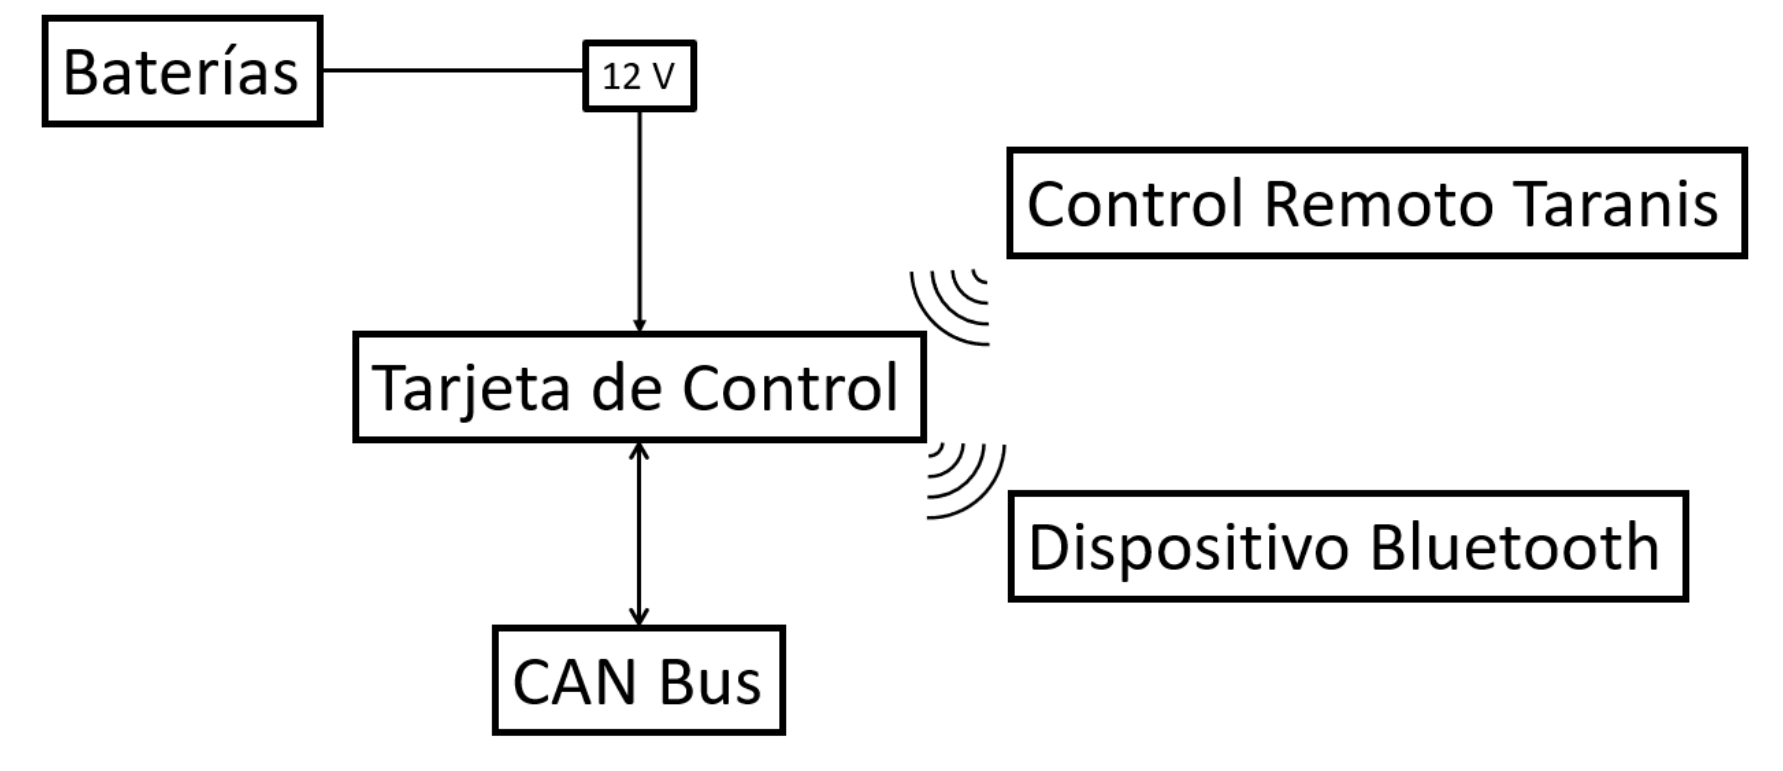
\includegraphics[width=0.8\textwidth]{figura6.png}
    \caption{Esquema general del Interprete CAN BT.}
    \label{fig:esquema_interprete}
\end{figure}

A través del esquema anterior, vemos cómo la tarjeta de control es capaz de recibir información del Control Remoto Taranis, y, opcionalmente, mandar información a través de Bluetooth, para monitorear la respuesta de cada uno de los sistemas del vehículo. Además, la tarjeta de control es la encargada de transformar toda la información que le llega en comandos CAN y enviarla de forma simultánea al resto de las placas.

Asimismo, para la realización del circuito impreso, fue necesario realizar el diagrama de caja negra de este sistema, el cual se muestra en la Fig. \ref{fig:caja_negra_interprete}.

\begin{figure}[H]
    \centering
    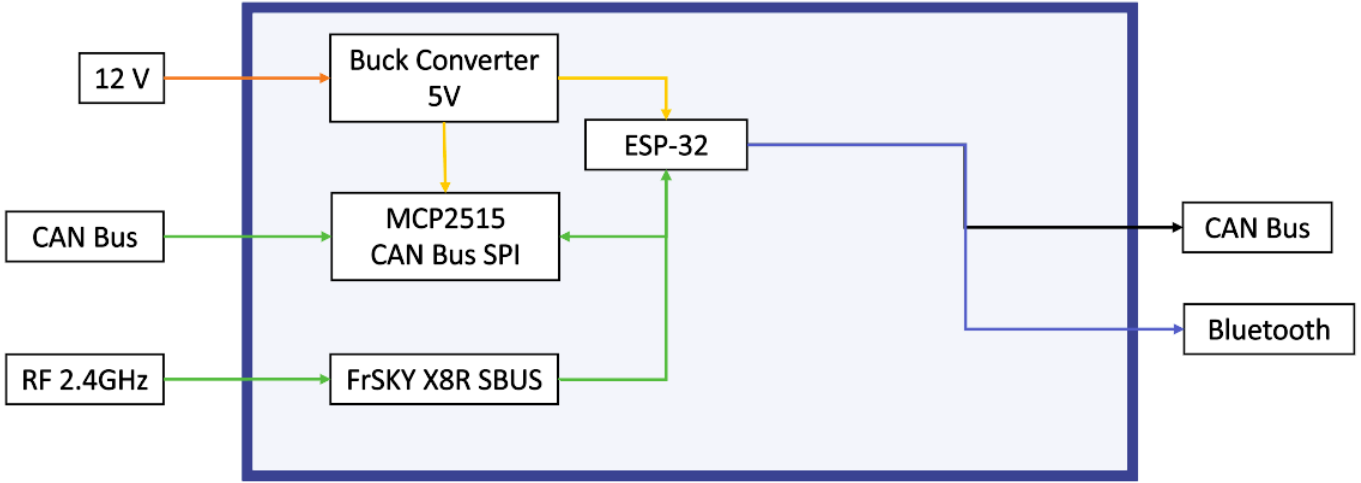
\includegraphics[width=0.8\textwidth]{figura7.png}
    \caption{Diagrama de Caja Negra de la PCB del Interprete CAN BT.}
    \label{fig:caja_negra_interprete}
\end{figure}

En el diagrama, podemos observar cómo la placa recibe alimentación de los 12 V de una de las baterías, la señal de radiofrecuencia del control remoto y las respuestas del resto de los sistemas en forma de comandos CAN. Toda esta información es procesada por un ESP32, el cual manda los comandos CAN, y también manda por Bluetooth si los sistemas están contestando adecuadamente.

Ya una vez definido lo anterior, se realizó el diagrama esquemático del circuito, el cual se presenta en la Fig. \ref{fig:esquematico_interprete}.

\begin{figure}[H]
    \centering
    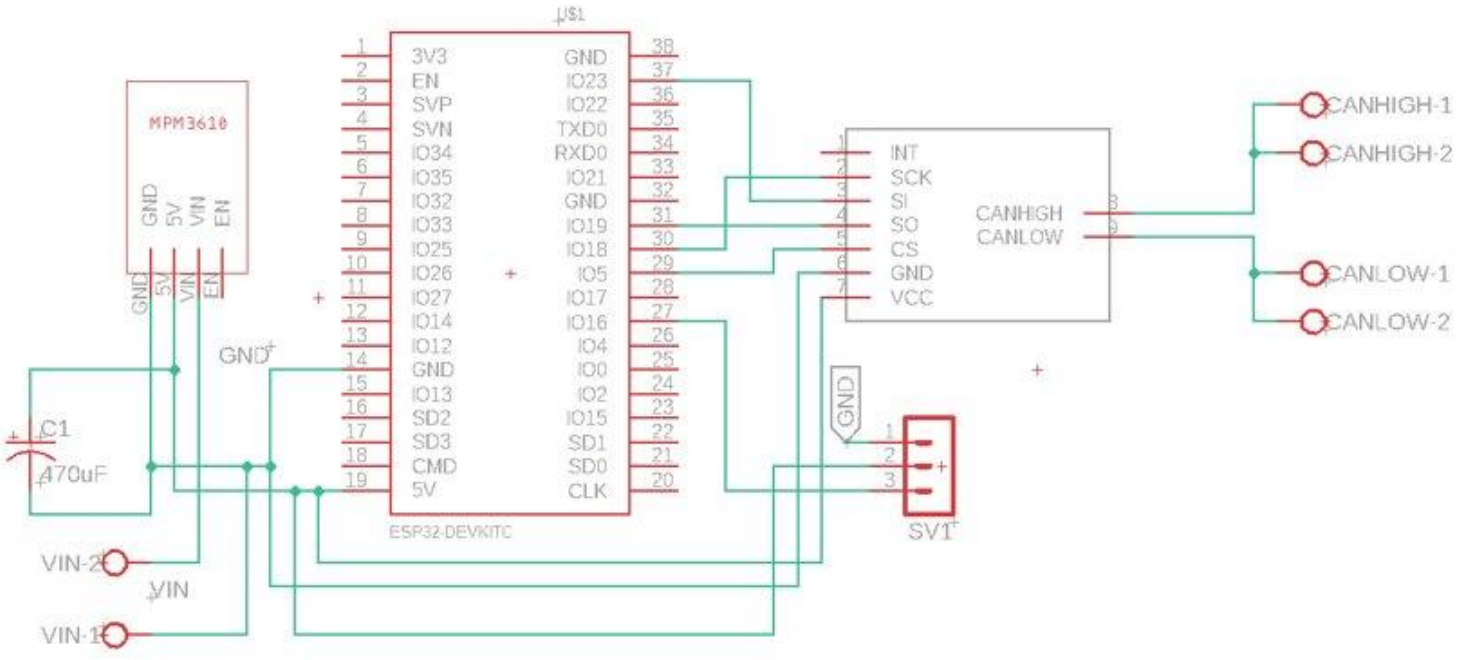
\includegraphics[width=1\textwidth]{figura8.png}
    \caption{Diagrama esquemático del circuito del Interprete CAN BT.}
    \label{fig:esquematico_interprete}
\end{figure}

A partir de éste, se realizó el diseño de la PCB (Fig. \ref{fig:pcb_interprete}) y se puede encontrar el archivo Gerber de esta en la \href{#}{siguiente carpeta}.

\begin{figure}[H]
    \centering
    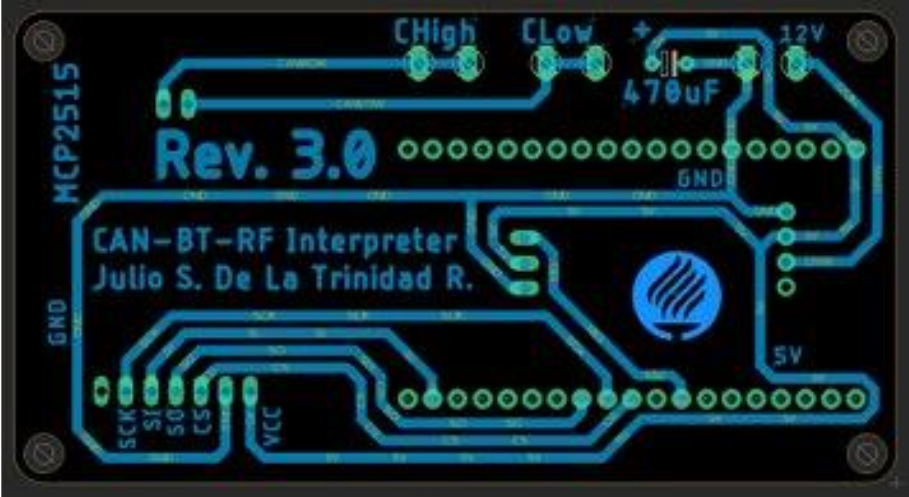
\includegraphics[width=0.7\textwidth]{figura9.png}
    \caption{PCB del circuito del Interprete CAN BT.}
    \label{fig:pcb_interprete}
\end{figure}

Para el circuito anterior es necesario contar con los componentes listados en la Tabla \ref{tab:comp_interprete}.

\begin{table}[H]
\centering
\caption{Lista de componentes del circuito del Interprete CAN BT}
\label{tab:comp_interprete}
\begin{tabular}{lllc}
\toprule
\textbf{CANTIDAD} & \textbf{ELEMENTO} & \textbf{Modelo} & \textbf{Link de compra} \\
\midrule
1 & Arduino Micro & Genérico & \href{#}{Arduino} \\
1 & Regulador 5 V & MPM3610 & \href{#}{Regulador} \\
3 & Clema 2 Posiciones & TB007 508 & \href{#}{Clemas} \\
1 & Resistencia 1k & Genérico & \href{#}{Resistencias} \\
1 & Resistencia 10k & Genérico & \href{#}{Resistencias} \\
1 & Modulo CAN Bus & MCP2515 & \href{#}{CAN} \\
1 & Capacitor (470uF) & Genérico & \href{#}{Capacitores} \\
\bottomrule
\end{tabular}
\end{table}

\subsubsection{Código}
Para la realización del código, se siguió la lógica del diagrama de flujo mostrado en la Fig. \ref{fig:flujo_interprete}. Por último, en el siguiente enlace se podrá encontrar el archivo ino, con el código utilizado para la implementación de este sistema \href{#}{Código}.

\begin{figure}[H]
    \centering
    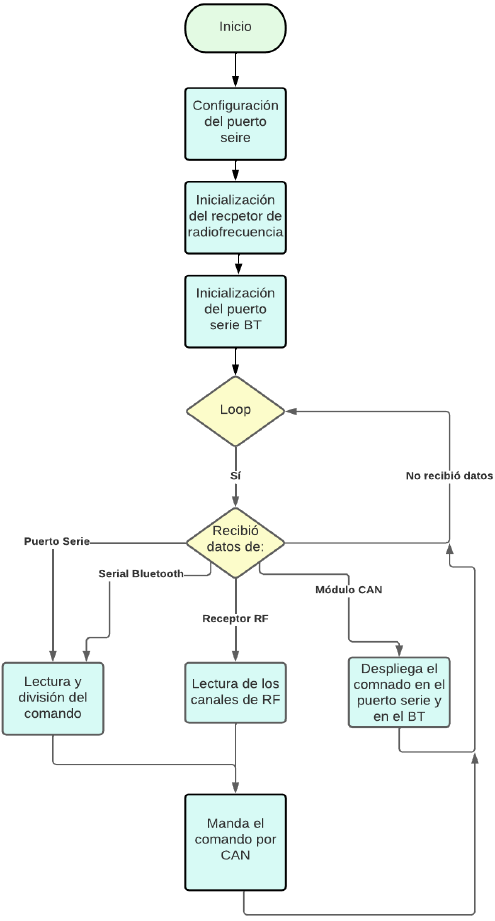
\includegraphics[width=0.6\textwidth]{figura10.png}
    \caption{Diagrama de flujo del programa de Interprete CAN.}
    \label{fig:flujo_interprete}
\end{figure}

\subsection{Tren motriz}
\label{sec:tren_motriz}

\begin{figure}[H]
    \centering
    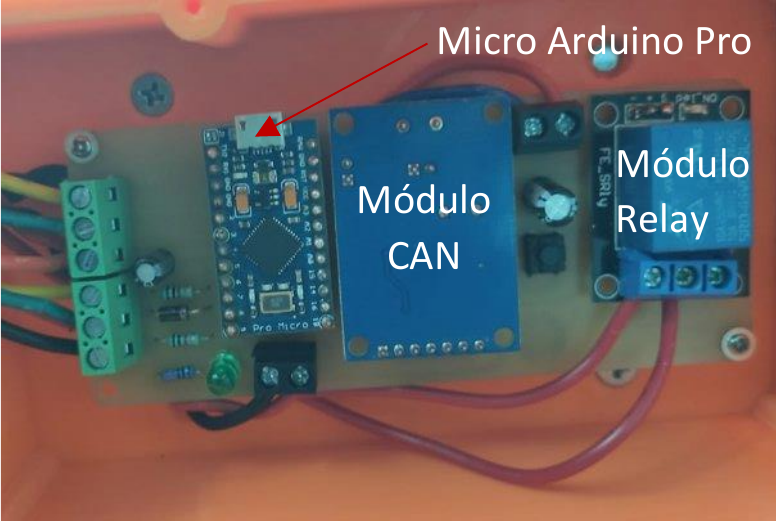
\includegraphics[width=0.6\textwidth]{figura11.png}
    \caption{Implementación del sistema de Tren motriz.}
    \label{fig:impl_tren_motriz}
\end{figure}

\begin{figure}[H]
    \centering
    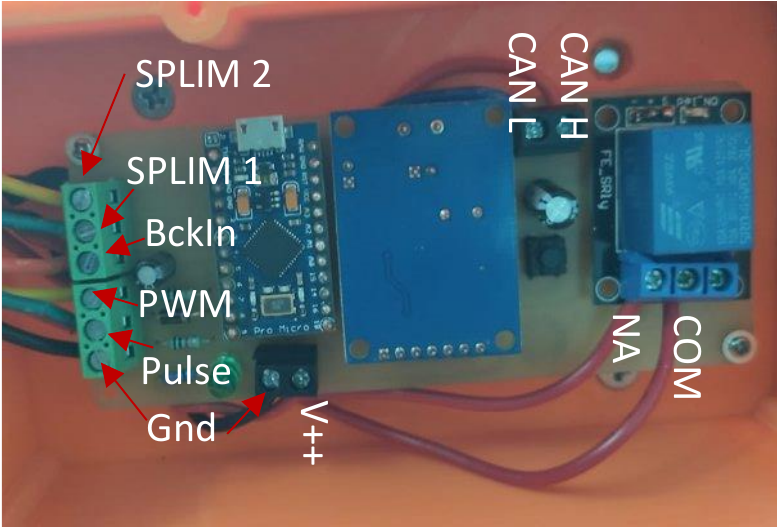
\includegraphics[width=0.6\textwidth]{figura12.png}
    \caption{Conexiones del sistema de Tren Motriz.}
    \label{fig:conexiones_tren_motriz}
\end{figure}

Ahora bien, el sistema de Tren motriz es el encargado de generar el movimiento en las llantas traseras del AMR, para que éste pueda desplazarse. Para esto, el sistema utiliza un conjunto de cuatro baterías conectadas en serie con el objetivo de generar 48 V de corriente directa, para alimentar al motor trifásico. Asimismo, se utiliza un controlador de 9 pines para poder obtener distintos comportamientos del motor, estos reciben la señal de un Arduino Micro Pro, que recibe los comandos CAN necesarios para hacer el control. Esto se puede apreciar en las figuras \ref{fig:bloques_tren} y \ref{fig:visual_tren}, en dónde se presenta el esquema general del tren motriz, así como el esquema visual del mismo, respectivamente.

\begin{figure}[H]
    \centering
    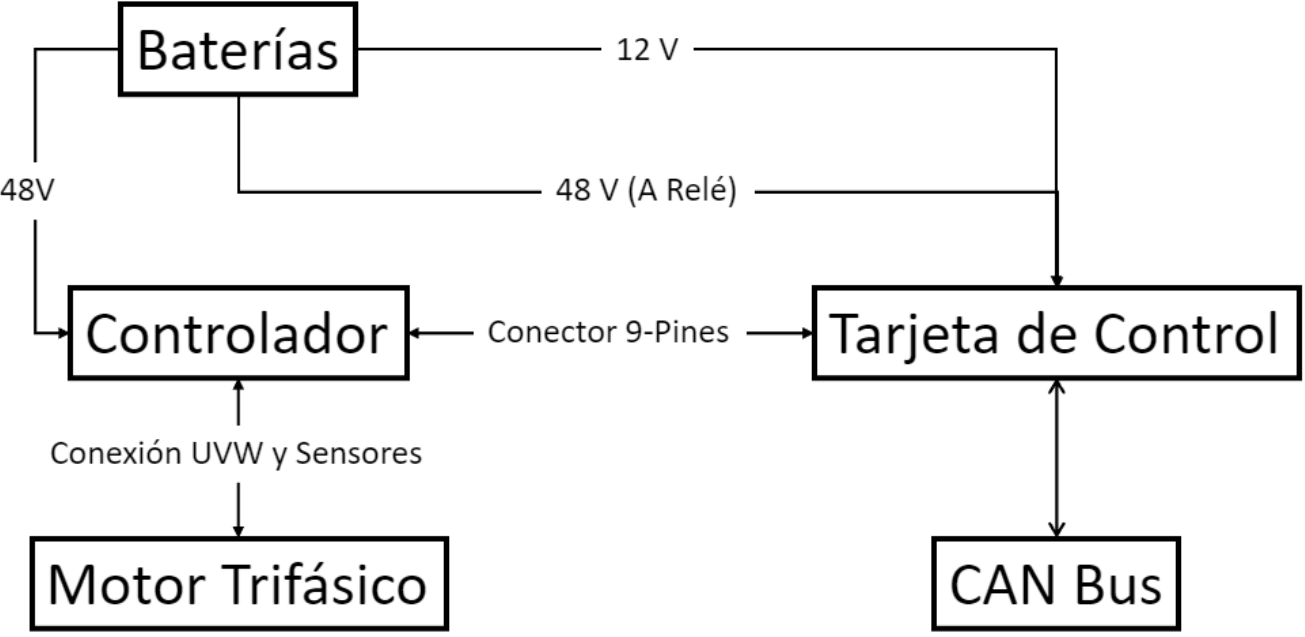
\includegraphics[width=0.8\textwidth]{figura13.png}
    \caption{Diagrama de bloques del sistema del Tren Motriz.}
    \label{fig:bloques_tren}
\end{figure}

\begin{figure}[H]
    \centering
    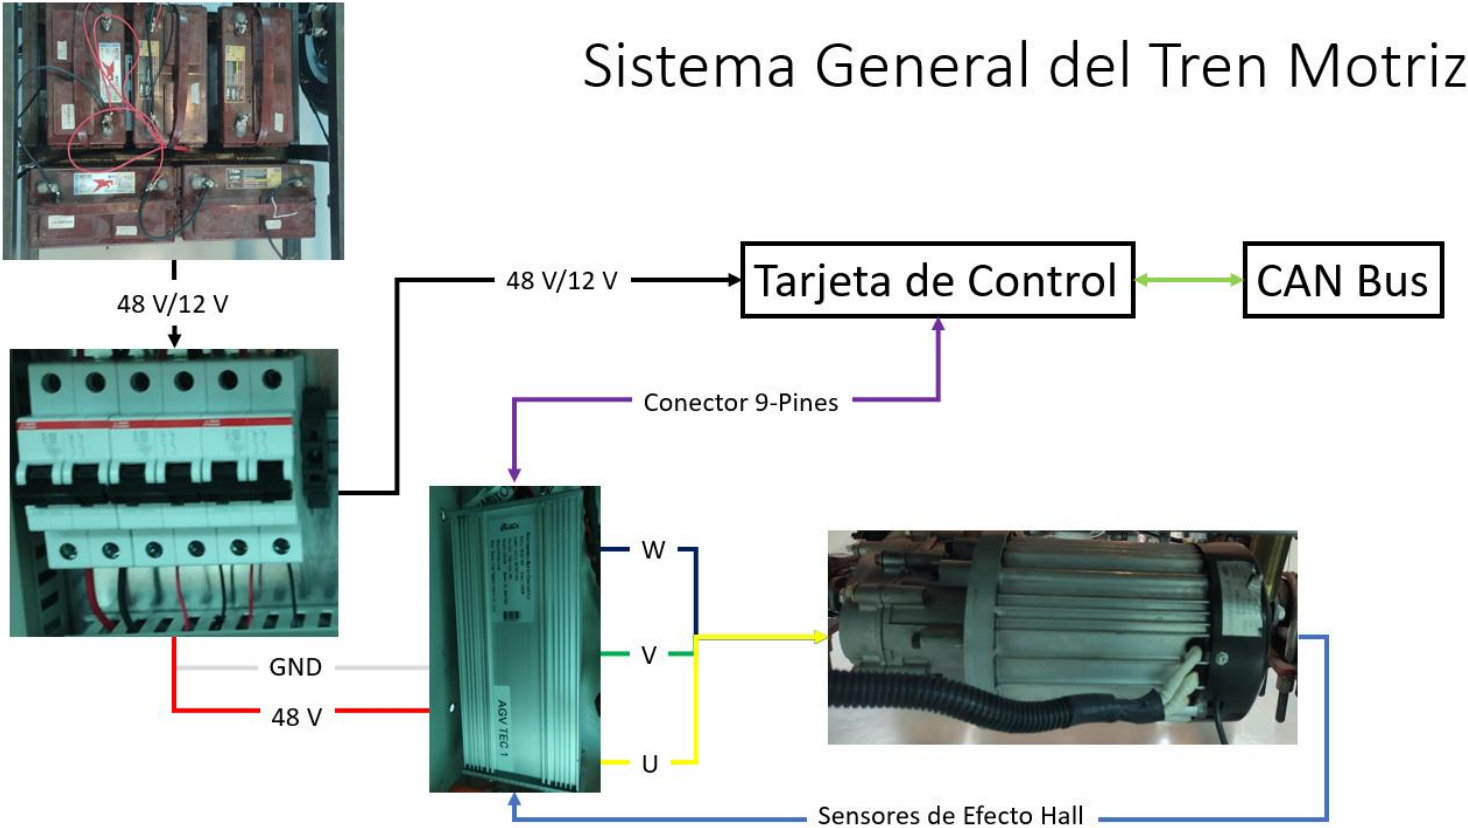
\includegraphics[width=0.8\textwidth]{figura14.png}
    \caption{Esquema visual del sistema general del Tren Motriz.}
    \label{fig:visual_tren}
\end{figure}

Para poder hacer el control del motor trifásico, se utiliza un controlador DC de 36 a 42 100 W, el cual hace uso de una conexión de 9 pines para controlar distintas funcionalidades del motor, entre las cuales están el Throttle, la velocidad límite, el pulso y el freno. Esto se puede ver representado de una forma más clara en la Fig. \ref{fig:especifico_controlador}.

\begin{figure}[H]
    \centering
    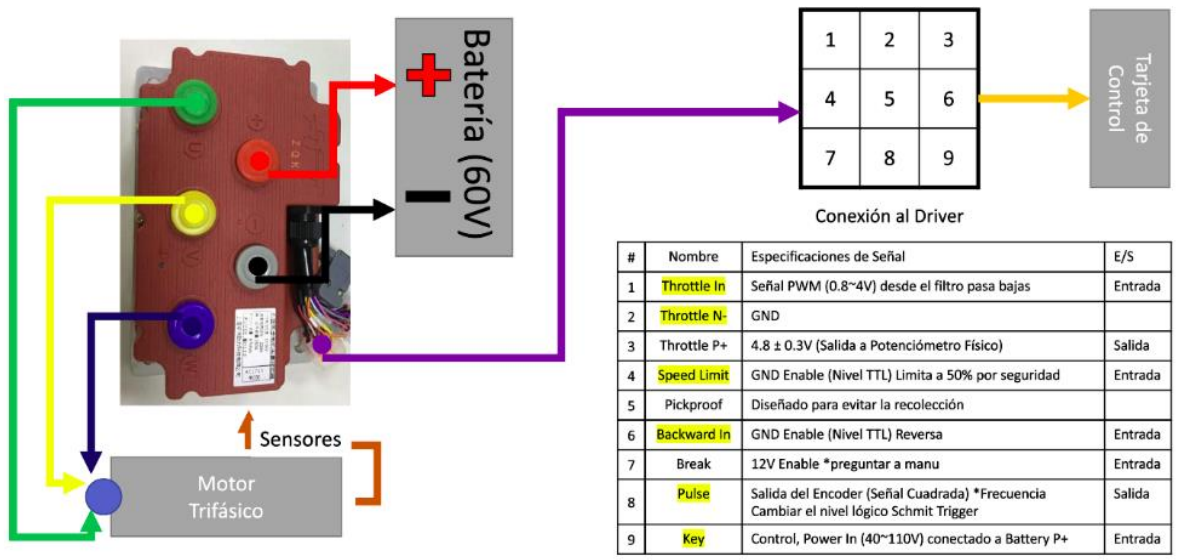
\includegraphics[width=1\textwidth]{figura15.png}
    \caption{Diagrama específico del controlador.}
    \label{fig:especifico_controlador}
\end{figure}

Una vez especificado lo anterior, se realizó el diagrama de caja negra de este sistema, en el cual podemos observar cómo la placa recibe como alimentación tanto 12 V como 48 V, y como señales recibe comandos CAN, pulsos de las RPM del driver del motor, y entradas auxiliares del mismo. Luego de esto, las señales son procesadas por el Arduino Nano Pro, y a la salida produce las señales para el controlador del motor, tal y cómo se ve en la Fig. \ref{fig:caja_negra_tren}. Además, hay que destacar que también se hace uso de un Relé normalmente abierto como sistema de seguridad, pues éste suministrará el voltaje al pin Lock del controlador, bloqueando el sistema.

\begin{figure}[H]
    \centering
    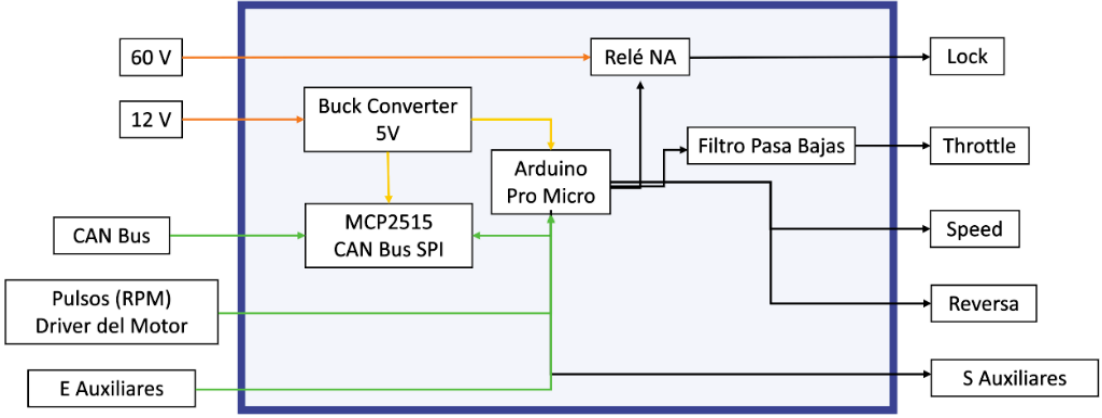
\includegraphics[width=0.9\textwidth]{figura16.png}
    \caption{Diagrama de Caja Negra de la PCB del Tren Motriz.}
    \label{fig:caja_negra_tren}
\end{figure}

\subsubsection{Placa de tren motriz de control}
Ya una vez definido lo anterior, se realizó el diagrama esquemático del circuito, el cual se presenta en la Fig. \ref{fig:esquematico_tren}.

\begin{figure}[H]
    \centering
    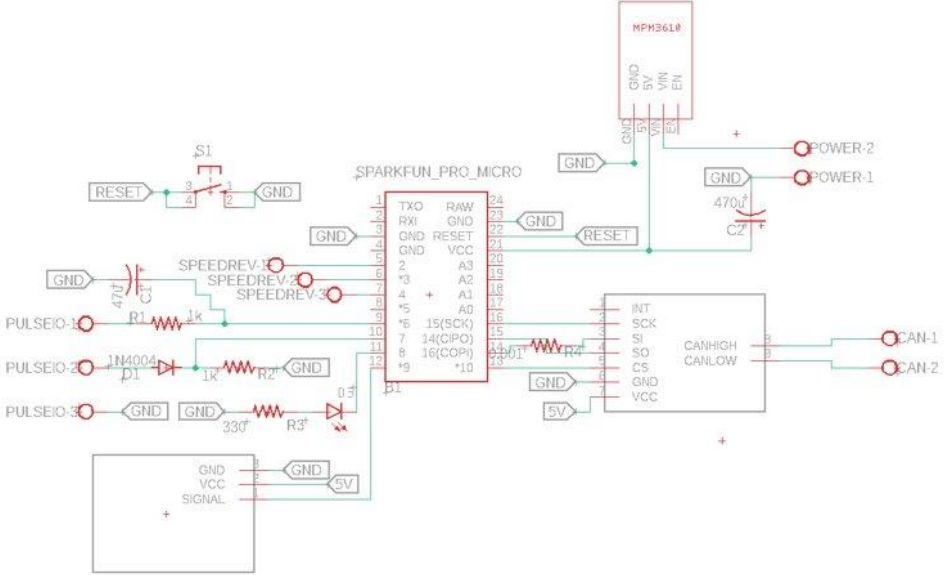
\includegraphics[width=1\textwidth]{figura17.png}
    \caption{Diagrama esquemático del circuito de Tren Motriz.}
    \label{fig:esquematico_tren}
\end{figure}

El diseño de la PCB se muestra en la Fig. \ref{fig:pcb_tren_control} y, en caso de ser necesario, puede encontrar el archivo Gerber de la misma en la \href{#}{siguiente carpeta}.

\begin{figure}[H]
    \centering
    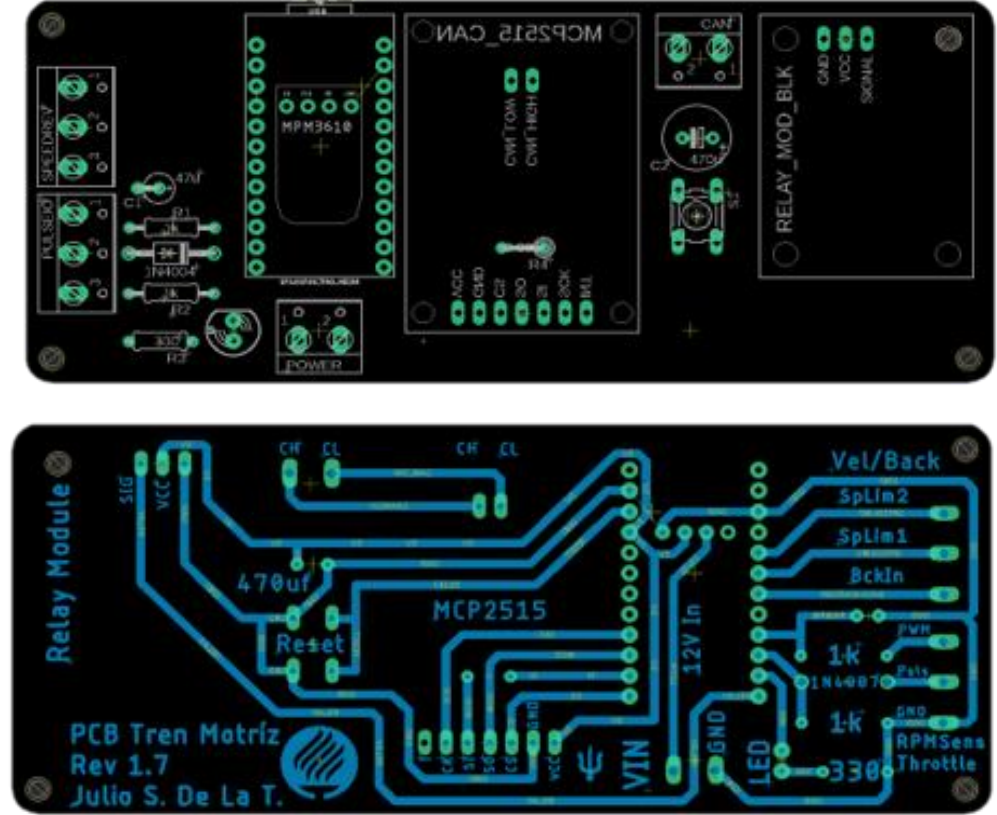
\includegraphics[width=0.8\textwidth]{figura18.png}
    \caption{PCB del circuito de Tren Motriz de control.}
    \label{fig:pcb_tren_control}
\end{figure}

Para poder realizar el circuito mencionado anteriormente, es necesario contar con la lista de componentes especificada en la Tabla \ref{tab:comp_tren_control}.

\begin{table}[H]
\centering
\caption{Lista de componentes del circuito del Tren Motriz de control}
\label{tab:comp_tren_control}
\begin{tabular}{lllc}
\toprule
\textbf{CANTIDAD} & \textbf{ELEMENTO} & \textbf{Modelo} & \textbf{Link de compra} \\
\midrule
1 & Arduino Micro & Genérico & \href{#}{Arduino} \\
1 & Regulador 5 V & MPM3610 & \href{#}{Regulador} \\
4 & Clema 2 Posiciones & TB007 508 & \href{#}{Clemas} \\
1 & Clema 3 Posiciones & TB007 508 & \href{#}{Clemas} \\
1 & Resistencia 330 & Genérico & \href{#}{Resistencias} \\
1 & Resistencia 1k & Genérico & \href{#}{Resistencias} \\
1 & Resistencia 10k & Genérico & \href{#}{Resistencias} \\
1 & LED & Genérico & \href{#}{Leds} \\
1 & Modulo CAN Bus & MCP2515 & \href{#}{CAN} \\
1 & Capacitor (470uF) & Genérico & \href{#}{Capacitores} \\
1 & Capacitor (47uF) & Genérico & \href{#}{Capacitores} \\
1 & Modulo Pololu 24v21 & 2995 & \href{#}{Pololu} \\
1 & Diodo & 1N4007 & \href{#}{Diodo} \\
1 & Módulo Relay & Fe\_srly & \href{#}{Relay} \\
\bottomrule
\end{tabular}
\end{table}

\subsubsection{Placa de tren motriz de protección}
Adicional a la placa presentada anteriormente, el tren motriz incluye una placa de protección para el Arduino Micro Pro, pues se llegó a detectar que existía una corriente que llegaba a uno de los pines de salida del Arduino, lo que provocaba que éste se quemara. Por lo tanto, se colocó el circuito adicional como forma de protección.

El diseño de la PCB se muestra a continuación en la Fig. \ref{fig:pcb_tren_proteccion}. Cabe mencionar que en este diseño se emplearon las huellas de un TIP42C, es necesario tomar en cuenta la ubicación de Base, Colector y Emisor del 2n2222.

\begin{figure}[H]
    \centering
    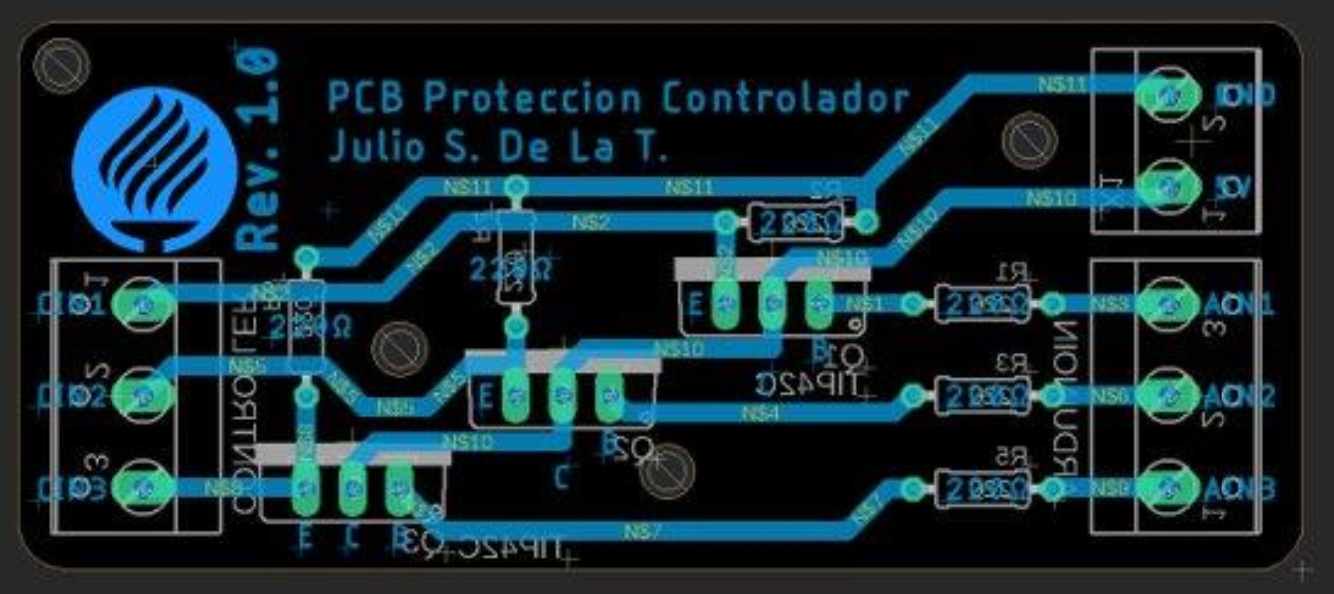
\includegraphics[width=0.8\textwidth]{figura19.png}
    \caption{PCB del circuito de Tren Motriz de protección.}
    \label{fig:pcb_tren_proteccion}
\end{figure}

El circuito mencionado anteriormente cuenta con los componentes especificados en la Tabla \ref{tab:comp_tren_proteccion}.

\begin{table}[H]
\centering
\caption{Lista de componentes del circuito del Tren Motriz de protección}
\label{tab:comp_tren_proteccion}
\begin{tabular}{lllc}
\toprule
\textbf{CANTIDAD} & \textbf{ELEMENTO} & \textbf{Modelo} & \textbf{Link de compra} \\
\midrule
1 & Clema 2 Posiciones & TB007 508 & \href{#}{Clemas} \\
3 & Clema 3 Posiciones & TB007 508 & \href{#}{Clemas} \\
3 & Resistencia 220 & Genérico & \href{#}{Resistencias} \\
3 & Transistor & 2n2222 & \href{#}{Resistencias} \\
\bottomrule
\end{tabular}
\end{table}

\subsubsection{Código}
Para la realización del código, se siguió la lógica del diagrama de flujo mostrado en la Fig. \ref{fig:flujo_tren}. A continuación se presenta el enlace en dónde se puede encontrar el archivo ino con el código utilizado para la implementación de este sistema \href{#}{Código}.

\begin{figure}[H]
    \centering
    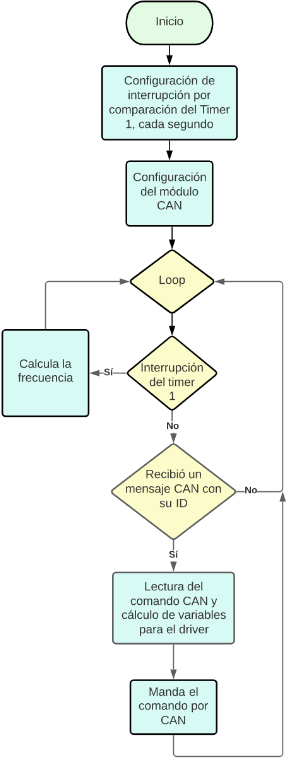
\includegraphics[width=0.6\textwidth]{figura20.png}
    \caption{Diagrama de flujo del programa de Tren Motriz.}
    \label{fig:flujo_tren}
\end{figure}

\subsection{Dirección}
\label{sec:direccion}
Como se describió anteriormente, el sistema de dirección cuenta con un motor DC que hace girar un sistema de engranes lo cual provoca que la dirección rote, cambiando la posición de las llantas. Los elementos mecánicos del sistema se indican en la Fig. \ref{fig:mec_direccion}.

\begin{figure}[H]
    \centering
    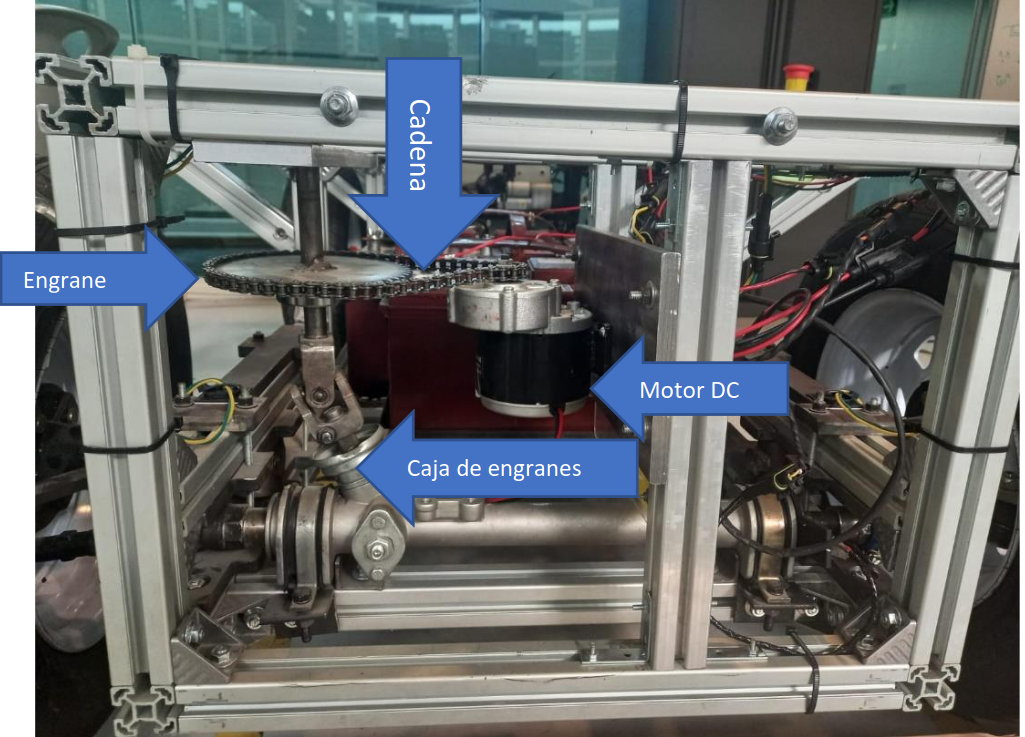
\includegraphics[width=0.7\textwidth]{figura21.png}
    \caption{Elementos mecánicos del sistema de dirección.}
    \label{fig:mec_direccion}
\end{figure}

Además, la parte electrónica del sistema se muestra en la Fig. \ref{fig:impl_direccion}.

\begin{figure}[H]
    \centering
    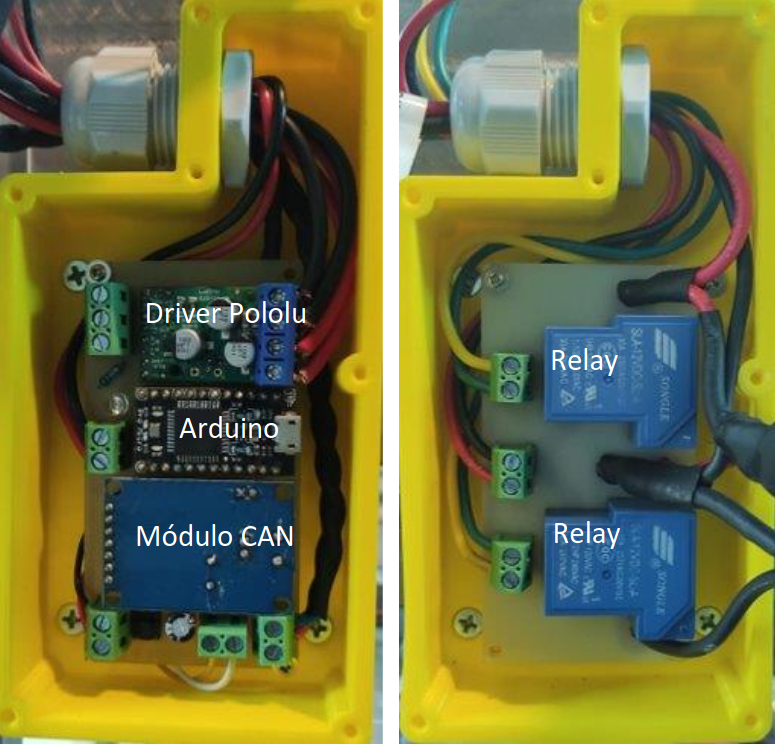
\includegraphics[width=0.7\textwidth]{figura22.png}
    \caption{Implementación del sistema de Dirección.}
    \label{fig:impl_direccion}
\end{figure}

\begin{figure}[H]
    \centering
    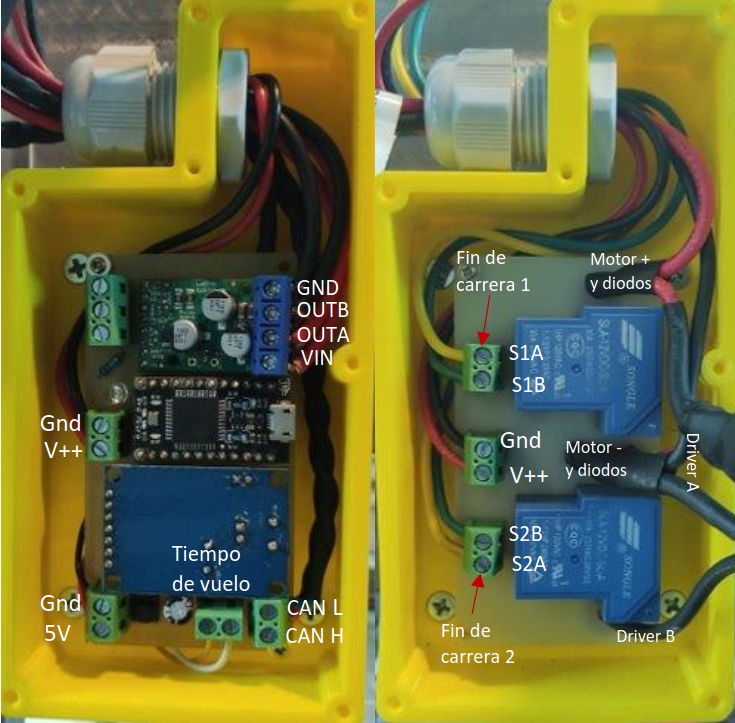
\includegraphics[width=0.7\textwidth]{figura23.png}
    \caption{Conexiones del sistema de Dirección.}
    \label{fig:conexiones_direccion}
\end{figure}

Con lo que respecta al sistema de dirección, podemos encontrar dos subsistemas principales. El primero de ellos es el encargado de recibir los comandos CAN del intérprete junto con los sensores de vuelo y mandar las señales pertinentes al controlador Pololu para hacer el control del motor de dirección. Por otra parte, el segundo subsistema es una placa de potencia, la cual recibe las señales del Pololu, y con base en unos sensores de fin de carrera bloquea el paso de la corriente en una dirección, con el objetivo de que, si alguna de las llantas llega al límite máximo que le permite el vehículo físicamente, ya no siga girando en ese sentido. Lo anterior se puede ver gráficamente en el esquema general de la dirección (Fig. \ref{fig:esquema_direccion}).

\begin{figure}[H]
    \centering
    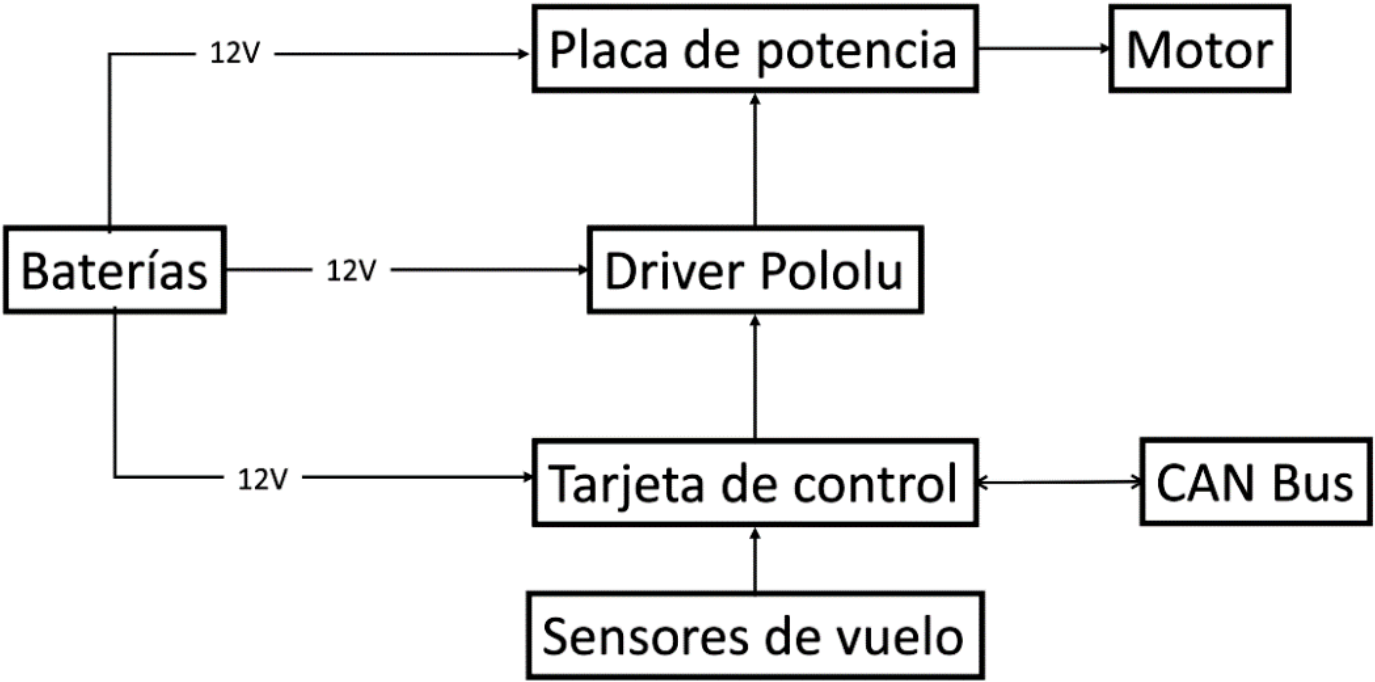
\includegraphics[width=0.8\textwidth]{figura24.png}
    \caption{Esquema general de la dirección.}
    \label{fig:esquema_direccion}
\end{figure}

Por lo tanto, para la realización del sistema de dirección, se implementaron dos circuitos impresos, uno para cada subsistema. A continuación, se presentan los diagramas de caja negra, los circuitos esquemáticos, los diseños de las PCB y la lista de materiales para cada uno de los subsistemas.

\subsubsection{Placa de CAN y control}
Esta placa es la encargada de recibir los comandos CAN del sistema de Intérprete CAN BT y con base en estos mandarle las señales pertinentes al Driver Pololu para poder controlar el motor de dirección. El diagrama de caja negra de éste se muestra en la Fig. \ref{fig:caja_negra_dir_control}.

\begin{figure}[H]
    \centering
    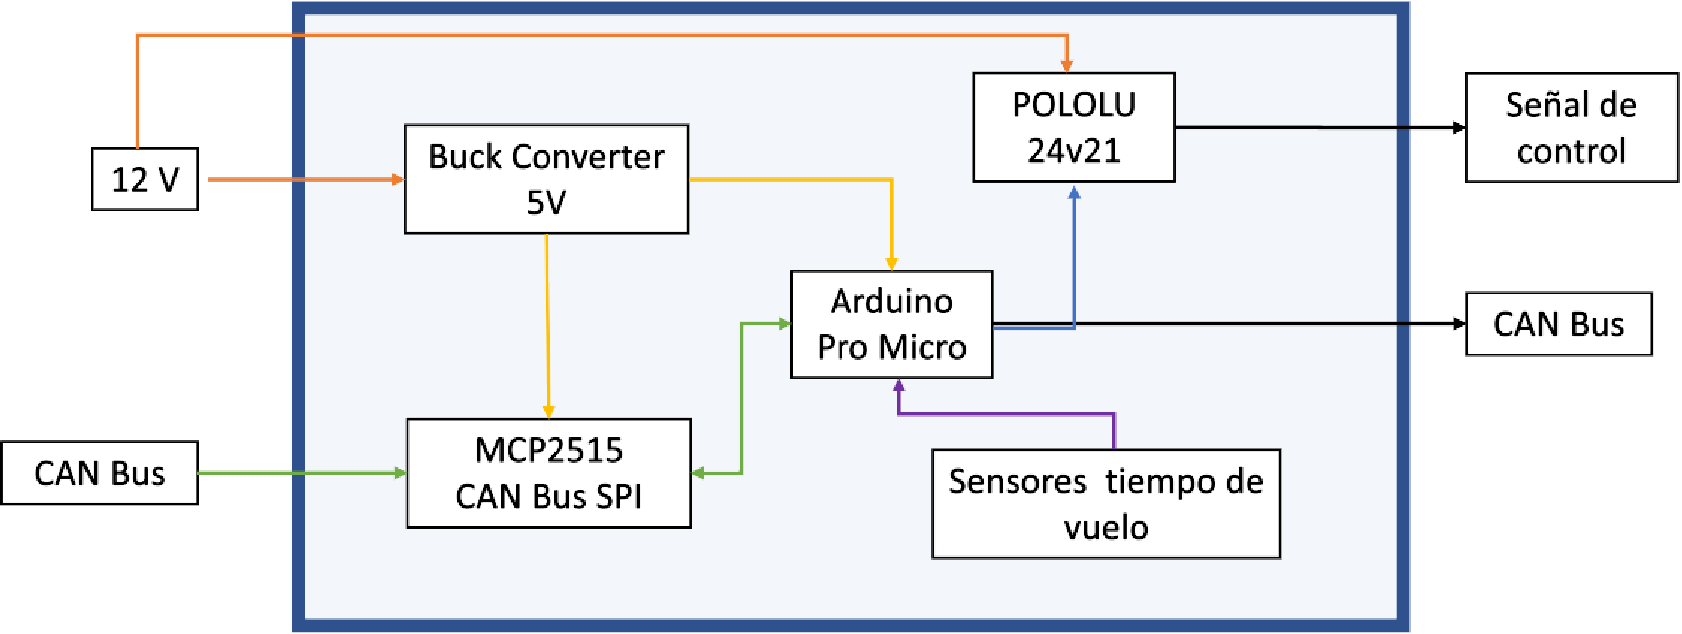
\includegraphics[width=0.9\textwidth]{figura25.png}
    \caption{Diagrama de Caja Negra de la PCB de dirección de CAN/Control.}
    \label{fig:caja_negra_dir_control}
\end{figure}

En ésta podemos observar que el sistema recibe como señales de entrada un voltaje de alimentación y comandos CAN de dirección; en estos comandos viene especificada la posición deseada a la que las llantas deben de llegar. Para lo anterior, el Arduino Pro Micro usa un sensor de tiempo de vuelo para detectar los grados de inclinación que tiene una de las llantas, y de esta forma hacer un sistema de control ON OFF con histéresis. Es importante aclarar que, si bien en el diagrama se coloca al sensor de tiempo de vuelo dentro de la caja, físicamente este se encuentra en la parte delantera en el perfil izquierdo del robot, a tan solo unos cuantos centímetros de la base.

Luego de esto, el Arduino manda un comando CAN de respuesta como salida y manda la señal pertinente a la tarjeta de potencia, para que ésta posteriormente permita o no su paso hacia el motor.

El diagrama esquemático del circuito se presenta en la Fig. \ref{fig:esquematico_dir_control}.

\begin{figure}[H]
    \centering
    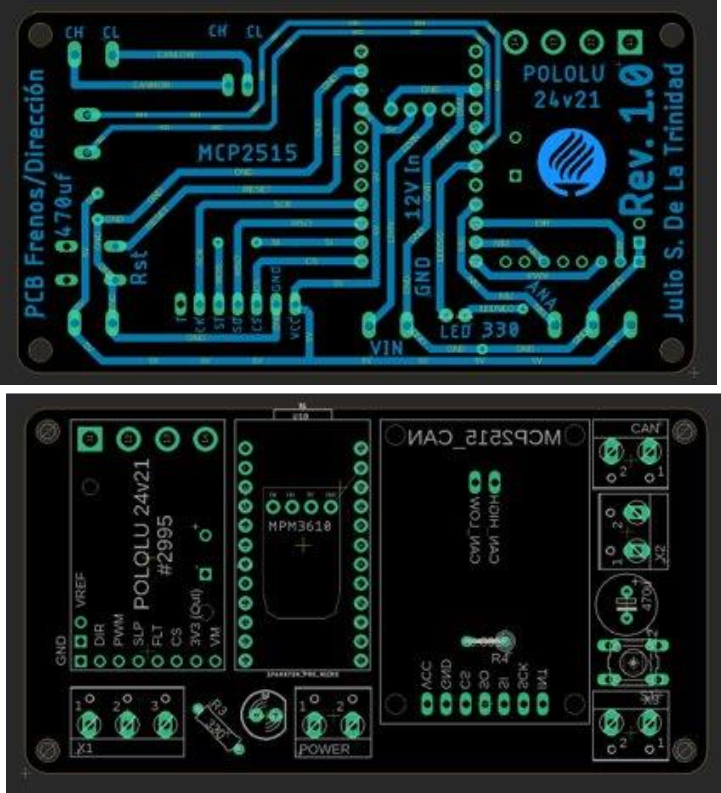
\includegraphics[width=1\textwidth]{figura26.png}
    \caption{Diagrama esquemático del circuito de dirección de CAN/Control.}
    \label{fig:esquematico_dir_control}
\end{figure}

A partir de éste, se realizó el diseño de la PCB (Fig. \ref{fig:pcb_dir_control}) y se puede encontrar su archivo Gerber en la \href{#}{siguiente carpeta}.

\begin{figure}[H]
    \centering
    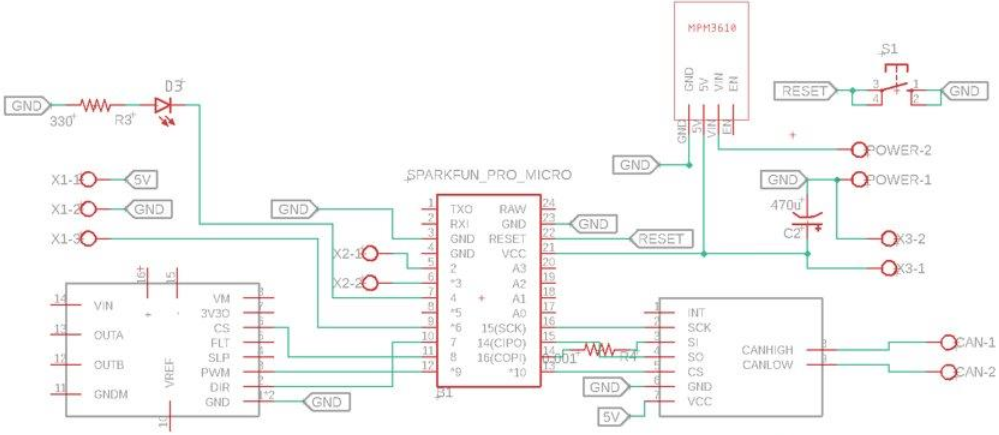
\includegraphics[width=0.8\textwidth]{figura27.png}
    \caption{PCB del circuito de dirección de CAN/CONTROL.}
    \label{fig:pcb_dir_control}
\end{figure}

Para el circuito mencionado, es necesario contar con los componentes especificados en la Tabla \ref{tab:comp_dir_control}.

\begin{table}[H]
\centering
\caption{Lista de componentes del circuito de Dirección de CAN/Control}
\label{tab:comp_dir_control}
\begin{tabular}{lllc}
\toprule
\textbf{CANTIDAD} & \textbf{ELEMENTO} & \textbf{Modelo} & \textbf{Link de compra} \\
\midrule
1 & Arduino Micro & Genérico & \href{#}{Arduino} \\
1 & Regulador 5 V & MPM3610 & \href{#}{Regulador} \\
4 & Clema 2 Posiciones & TB007 508 & \href{#}{Clemas} \\
1 & Clema 3 Posiciones & TB007 508 & \href{#}{Clemas} \\
1 & Resistencia 330 & Genérico & \href{#}{Resistencias} \\
1 & LED & Genérico & \href{#}{Leds} \\
1 & Modulo CAN Bus & MCP2515 & \href{#}{CAN} \\
1 & Capacitor (470uF) & Genérico & \href{#}{Capacitores} \\
1 & Push Button & Genérico & \href{#}{Botón} \\
1 & Módulo Pololu 24v21 & 2995 & \href{#}{Pololu} \\
\bottomrule
\end{tabular}
\end{table}

\subsubsection{Placa de Potencia}
Esta placa juega un papel muy importante en cuestión de seguridad, pues es la encargada de permitir o no el paso de la corriente hacia el motor que controla la dirección. El diagrama de caja negra de este sistema se muestra en la Fig. \ref{fig:caja_negra_dir_potencia}.

\begin{figure}[H]
    \centering
    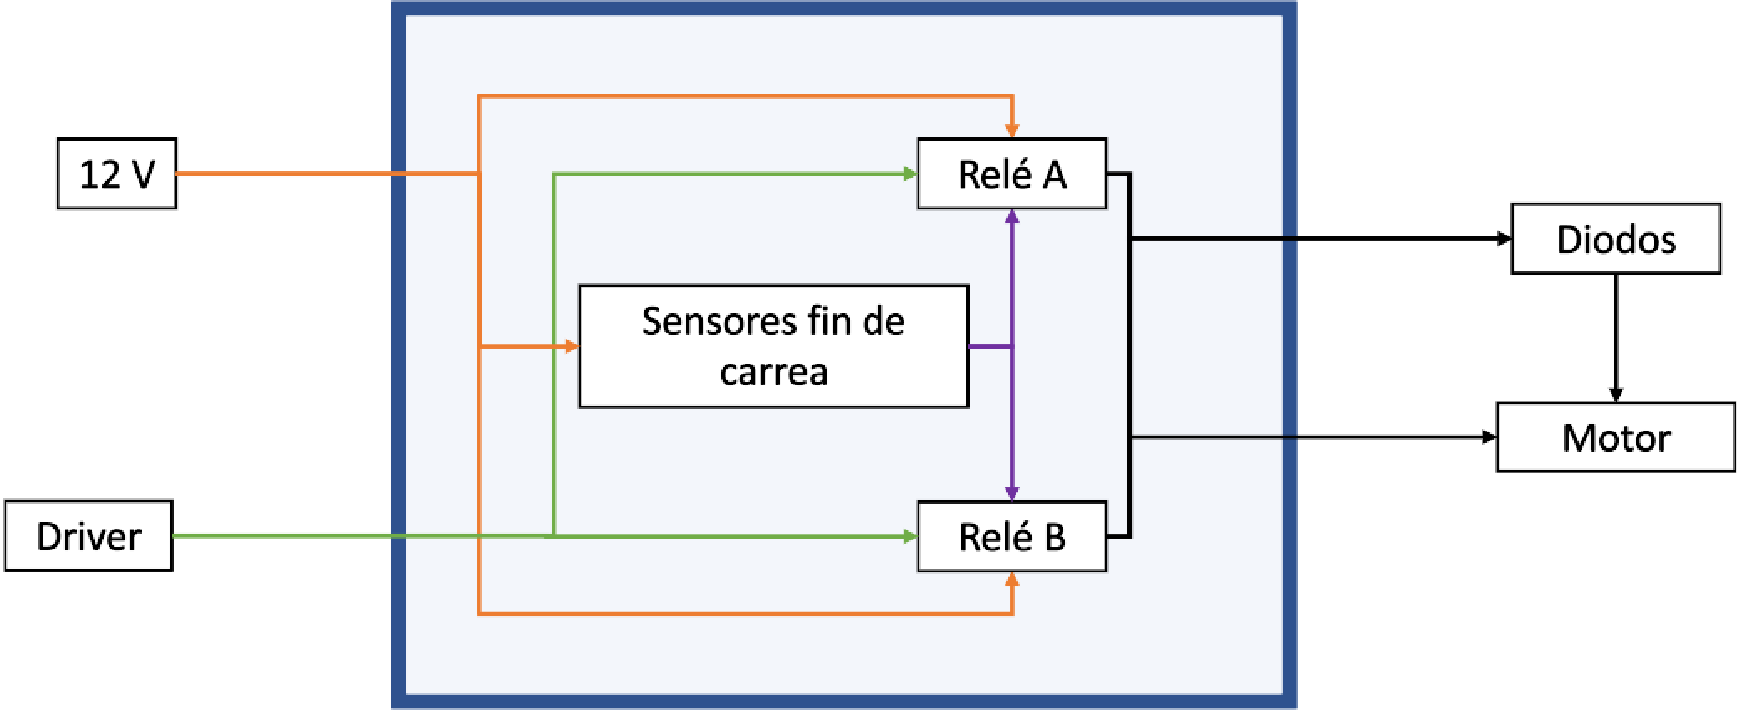
\includegraphics[width=0.8\textwidth]{figura28.png}
    \caption{Diagrama de Caja Negra de la PCB de dirección de Potencia.}
    \label{fig:caja_negra_dir_potencia}
\end{figure}

En ésta podemos observar que el sistema recibe como señales de entrada un voltaje de alimentación y la señal del controlador Pololu con la cual se determina el giro del motor. Ambas señales del controlador Pololu se conectan al pin normalmente abierto de cada uno de los relevadores.

Ahora bien, a cada una de las bobinas de los relevadores, están conectados los sensores de fin de carrera. En el momento en el que se presione uno de los dos sensores de fin de carrera, éste dejará de mandar 12 V a su respectivo relevador.

A continuación se presenta el diagrama esquemático.

\begin{figure}[H]
    \centering
    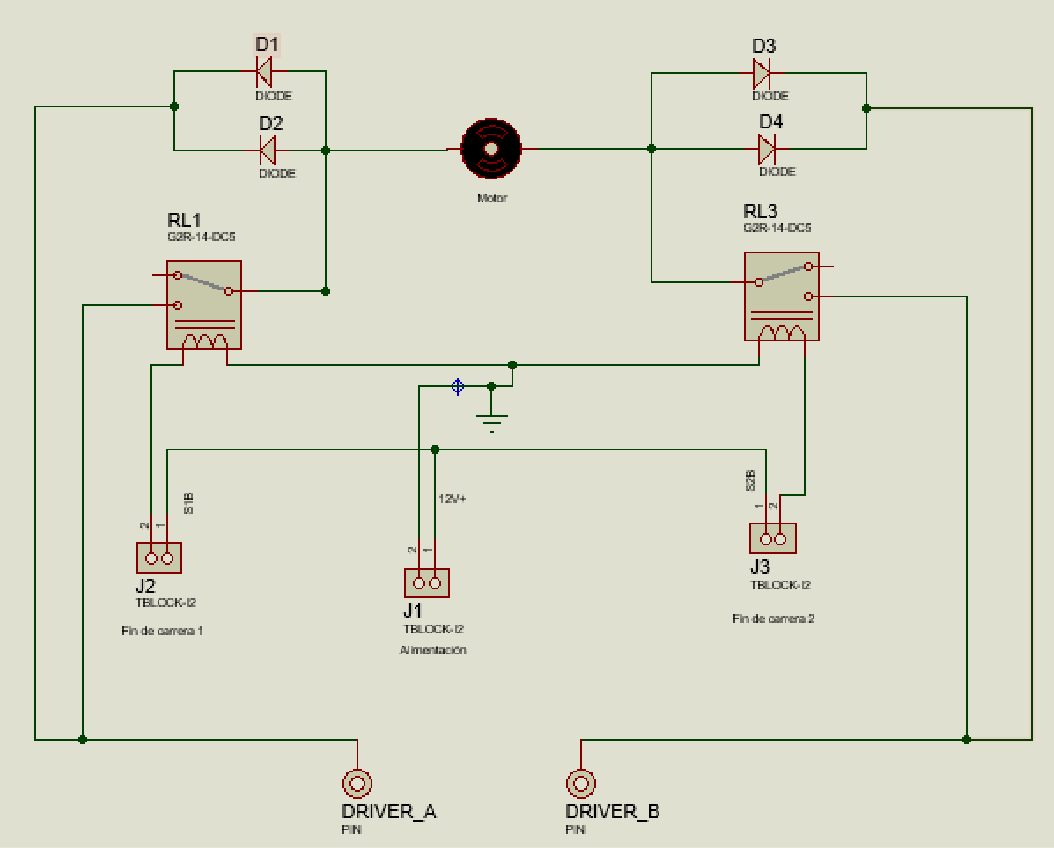
\includegraphics[width=1\textwidth]{figura29.png}
    \caption{Diagrama esquemático del circuito de dirección de potencia.}
    \label{fig:esquematico_dir_potencia}
\end{figure}

El diseño de la PCB se muestra a continuación en la Fig. \ref{fig:pcb_dir_potencia} y se puede encontrar su archivo Gerber en la \href{#}{siguiente carpeta}.

\begin{figure}[H]
    \centering
    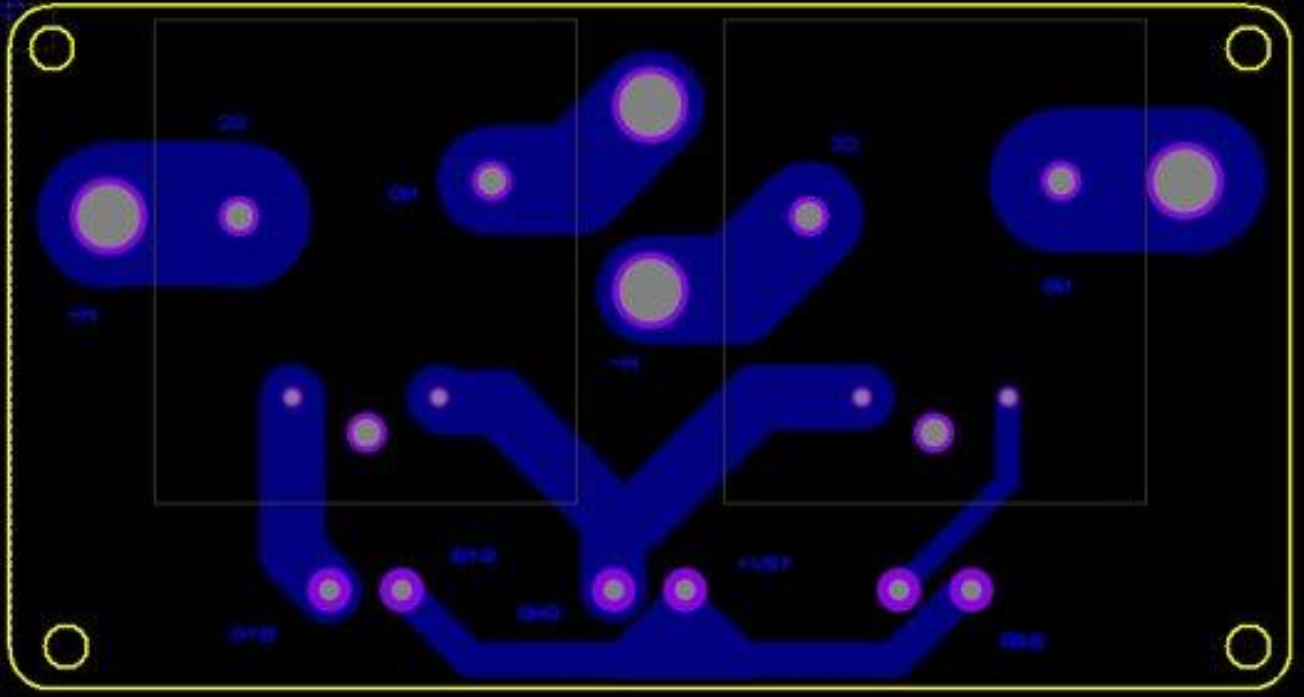
\includegraphics[width=0.8\textwidth]{figura30.png}
    \caption{PCB del circuito de dirección de Potencia.}
    \label{fig:pcb_dir_potencia}
\end{figure}

Componentes requeridos en la Tabla \ref{tab:comp_dir_potencia}.

\begin{table}[H]
\centering
\caption{Lista de componentes del circuito de Dirección de potencia}
\label{tab:comp_dir_potencia}
\begin{tabular}{lllc}
\toprule
\textbf{CANTIDAD} & \textbf{ELEMENTO} & \textbf{Modelo} & \textbf{Link de compra} \\
\midrule
2 & Relay 5 pines & sla 12vdc sl a & \href{#}{Relay} \\
1 & Borneras 2 pines grande & TB010 508 & \href{#}{Clemas} \\
2 & Borneras 2 pines mediana & TB007 508 & \href{#}{Clemas} \\
4 & Diodos & 10A10 & \href{#}{Diodo} \\
2 & Sensor fin de carrera & VS15 & \href{#}{Fin de carrera} \\
1 & Cable calibre 12 & Genérico & \href{#}{Cable} \\
1 & Cable calibre 16 & Genérico & \href{#}{Cable} \\
\bottomrule
\end{tabular}
\end{table}

\subsubsection{Código}
Diagrama de flujo mostrado en la Fig. \ref{fig:flujo_direccion}. A continuación se presenta el enlace en dónde se puede encontrar el archivo ino con el código utilizado para la implementación de este sistema \href{#}{Código}.

\begin{figure}[H]
    \centering
    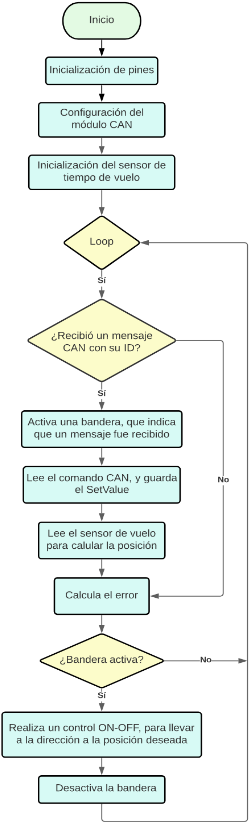
\includegraphics[width=0.6\textwidth]{figura31.png}
    \caption{Diagrama de flujo del programa de Dirección.}
    \label{fig:flujo_direccion}
\end{figure}

\subsection{Frenos}
\label{sec:frenos}
A continuación, se presenta una imagen del sistema de frenos, en dónde se señalan sus componentes mecánicos más importantes (ver Fig. \ref{fig:mec_frenos}).

\begin{figure}[H]
    \centering
    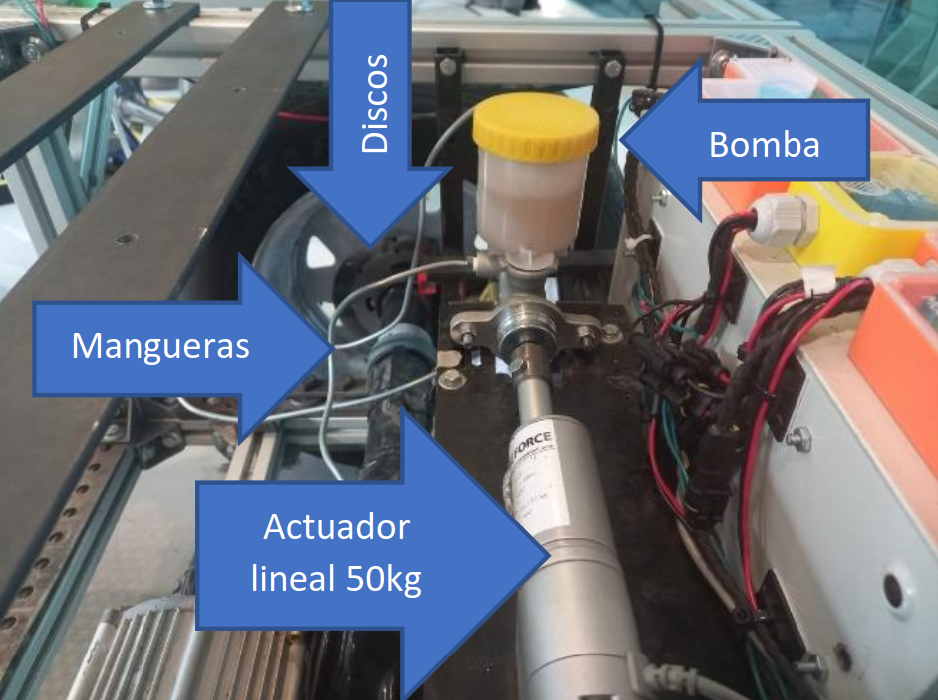
\includegraphics[width=0.7\textwidth]{figura32.png}
    \caption{Elementos mecánicos del sistema de frenos.}
    \label{fig:mec_frenos}
\end{figure}

Además, se muestran los subsistemas electrónicos implementados.

\begin{figure}[H]
    \centering
    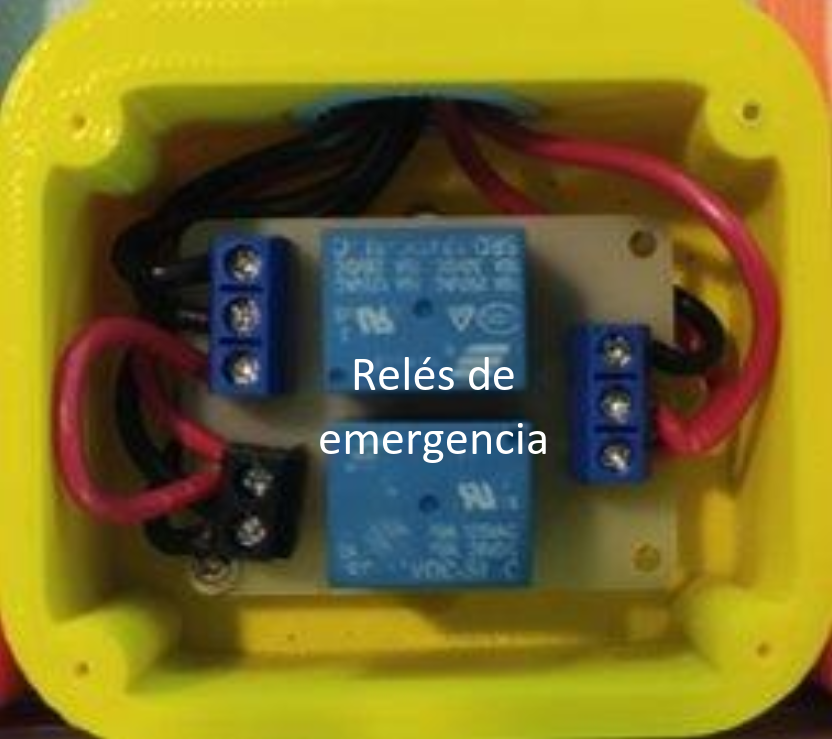
\includegraphics[width=0.7\textwidth]{figura33.png}
    \caption{Implementación del sistema de frenos.}
    \label{fig:impl_frenos}
\end{figure}

\begin{figure}[H]
    \centering
    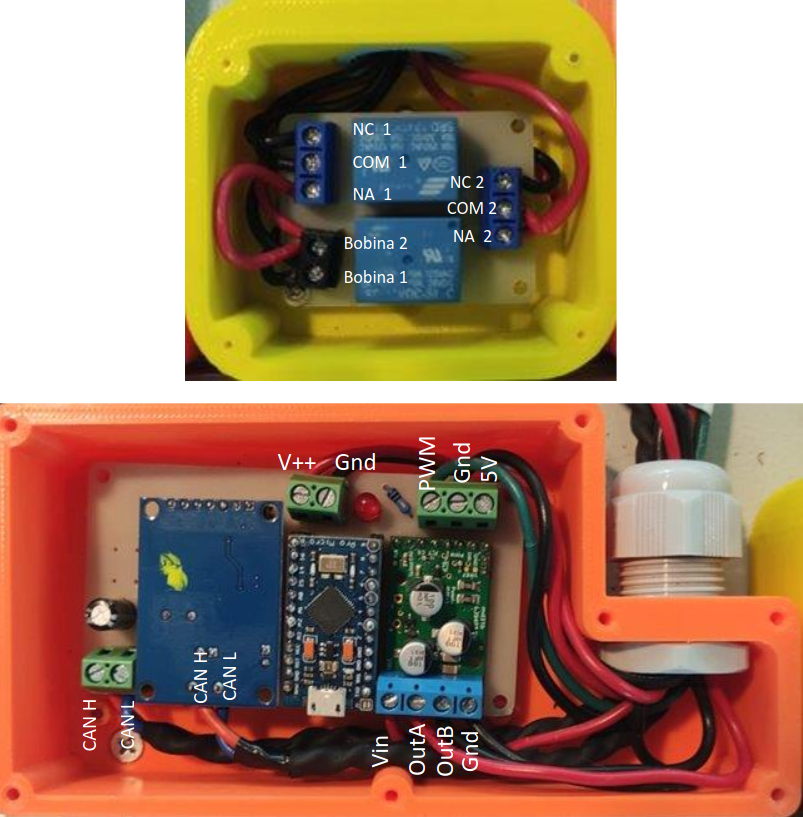
\includegraphics[width=0.7\textwidth]{figura34.png}
    \caption{Conexiones del sistema de Frenos.}
    \label{fig:conexiones_frenos}
\end{figure}

A continuación, se presenta el sistema general (Fig. \ref{fig:gen_frenos}), el diagrama de caja negra (Fig. \ref{fig:caja_negra_frenos}), el diagrama esquemático (Fig. \ref{fig:esquematico_frenos}) y los archivos correspondientes de la PCB (Fig. \ref{fig:pcb_frenos}).

\begin{figure}[H]
    \centering
    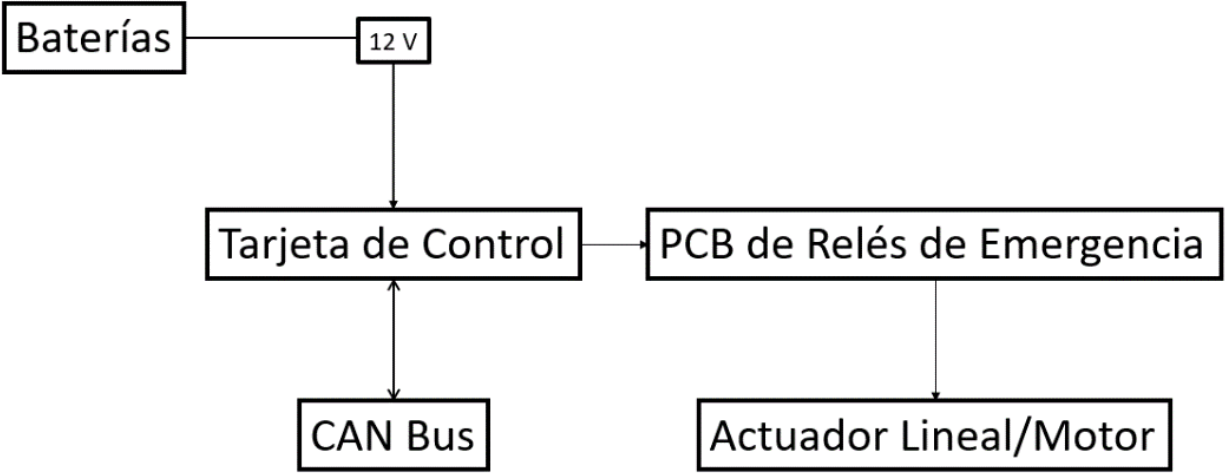
\includegraphics[width=0.8\textwidth]{figura35.png}
    \caption{Sistema general del control de frenos.}
    \label{fig:gen_frenos}
\end{figure}

\begin{figure}[H]
    \centering
    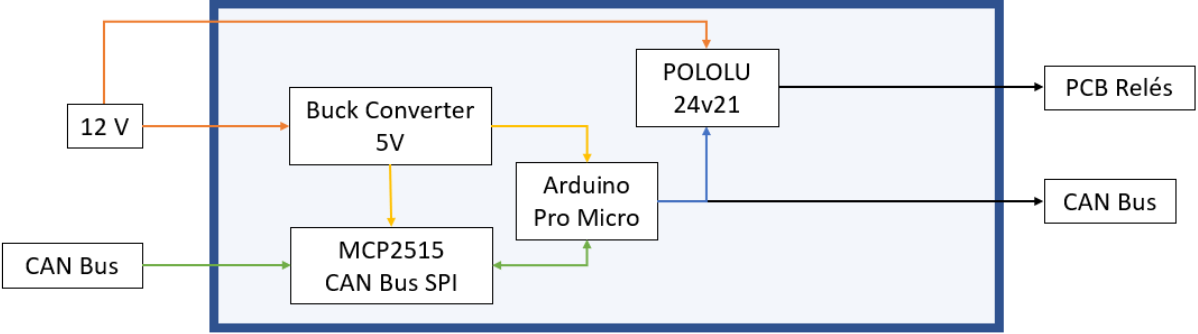
\includegraphics[width=0.9\textwidth]{figura36.png}
    \caption{Diagrama de caja negra del sistema de frenos.}
    \label{fig:caja_negra_frenos}
\end{figure}

\begin{figure}[H]
    \centering
    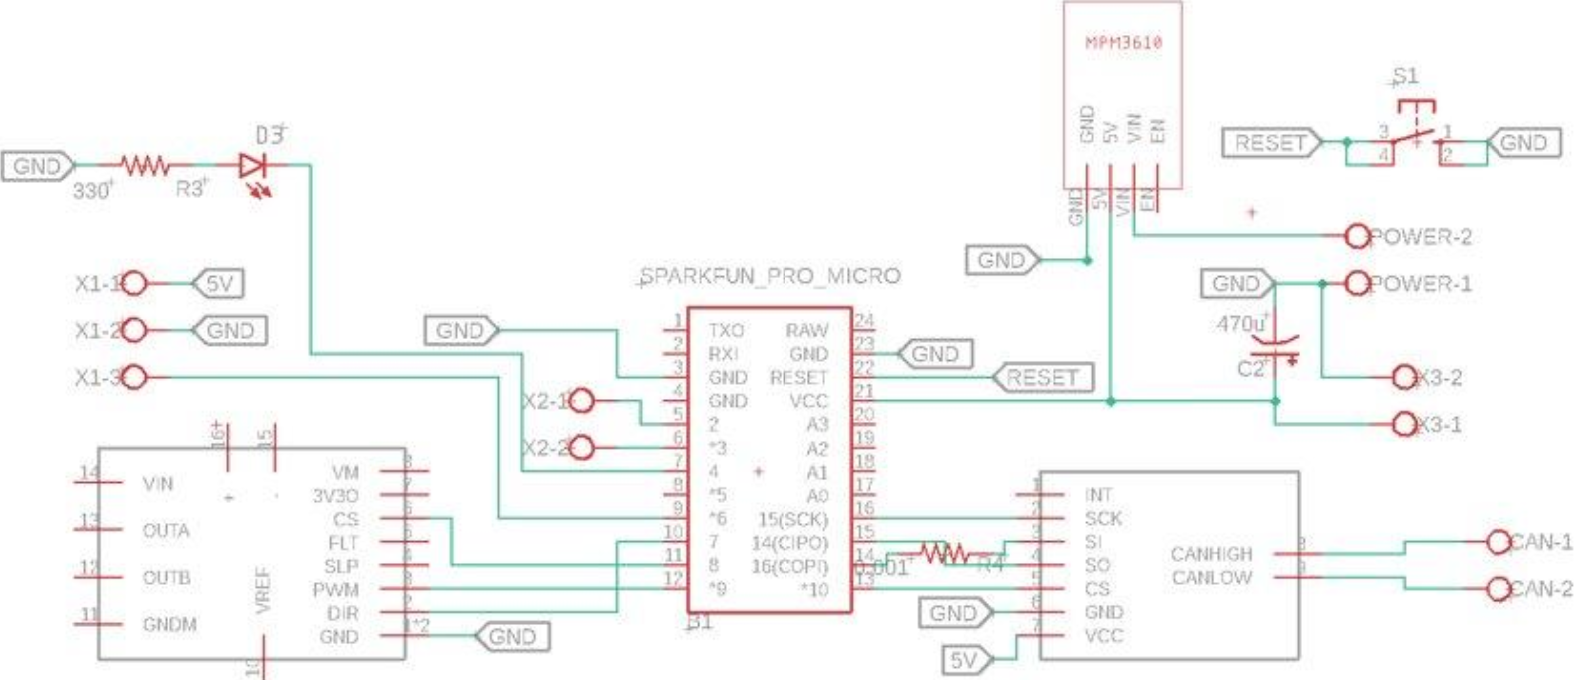
\includegraphics[width=1\textwidth]{figura37.png}
    \caption{Diagrama esquemático del sistema de frenos.}
    \label{fig:esquematico_frenos}
\end{figure}

\begin{figure}[H]
    \centering
    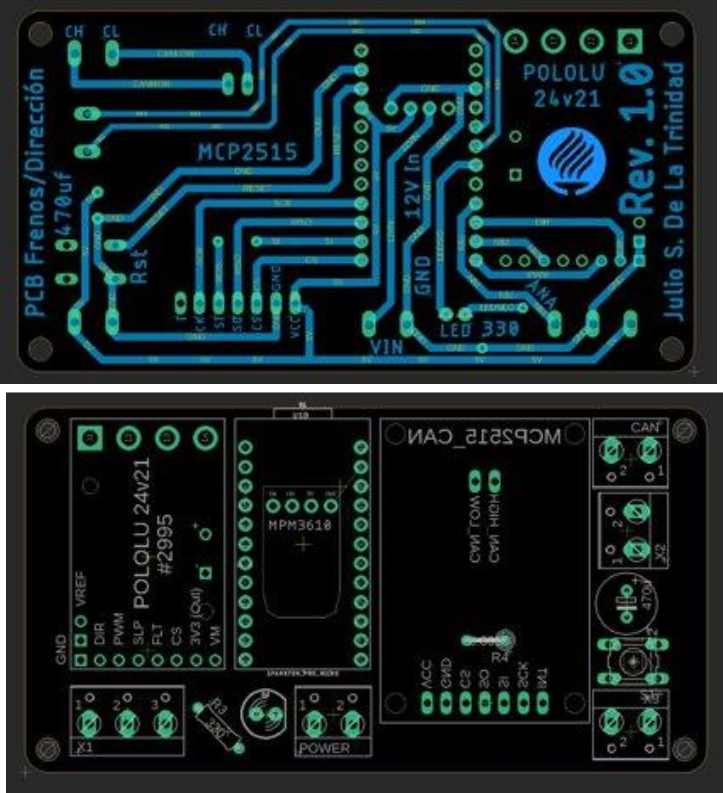
\includegraphics[width=0.8\textwidth]{figura38.png}
    \caption{Diseño de la PCB del sistema de frenos.}
    \label{fig:pcb_frenos}
\end{figure}

Lista de componentes especificada en la Tabla \ref{tab:comp_frenos}.

\begin{table}[H]
\centering
\caption{Lista de componentes para la PCB del sistema de frenos.}
\label{tab:comp_frenos}
\begin{tabular}{cl}
\toprule
\textbf{CANTIDAD} & \textbf{ELEMENTO} \\
\midrule
1 & Arduino Micro \\
1 & Regulador 5 V (MPM3610) \\
4 & Clema 2 Posiciones \\
1 & Clema 3 Posiciones \\
1 & Resistencia 330 \\
1 & LED \\
1 & Modulo CAN Bus (MCP2515) \\
1 & Capacitor (470uF) \\
1 & Push Button \\
1 & Modulo Pololu 24v21 \#2995 \\
\bottomrule
\end{tabular}
\end{table}

\subsubsection{Código}
Diagrama de flujo mostrado en la Fig. \ref{fig:flujo_frenos}. En el siguiente enlace se encuentra el \href{#}{Código}.

\begin{figure}[H]
    \centering
    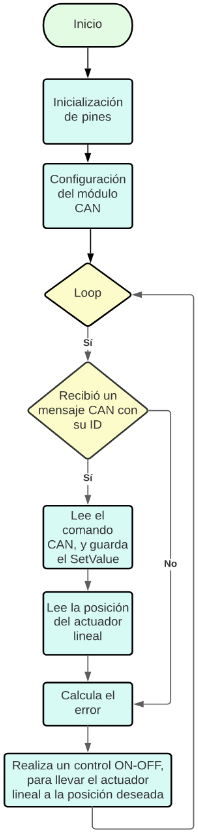
\includegraphics[width=0.6\textwidth]{figura39.png}
    \caption{Diagrama de flujo del programa de Frenos.}
    \label{fig:flujo_frenos}
\end{figure}

\subsection{Arneses}
Los arneses son el conjunto de circuitos (cables, terminales, conectores, cintas, entre otros) que llevan una señal de un punto a otro.

\subsubsection{Cables}
De manera general, se usaron cables de distinto color para hacer más sencillo identificar el tipo de señal. Se resume en la Tabla \ref{tab:guia_colores}.

\begin{table}[H]
\centering
\caption{Guía general de los colores de cable usados en el AMR1.}
\label{tab:guia_colores}
\begin{tabular}{ll}
\toprule
\textbf{Color de cable} & \textbf{Señal} \\
\midrule
Rojo & V++ \\
Negro & GND \\
Naranja & CAN High \\
Azul & CAN Low \\
Verde & Varias \\
Amarillo & Varias \\
\bottomrule
\end{tabular}
\end{table}

Calibres de cable utilizados en la Tabla \ref{tab:calibres_cable}.

\begin{table}[H]
\centering
\caption{Guía general de los calibres de cable usados en el AMR1.}
\label{tab:calibres_cable}
\begin{tabular}{lc}
\toprule
\textbf{Señal} & \textbf{Calibre del cable} \\
\midrule
Baterías & 8 \\
Alimentación & 14 \\
Motor Tren Motriz & 12 \\
CAN & 16 \\
Señales de sensores & 16 \\
Actuador lineal & 16 \\
Motor dirección & 12 \\
\bottomrule
\end{tabular}
\end{table}

\subsubsection{Conectores}
El proceso de ponchado de cables se muestra en la Fig. \ref{fig:ponchado}.

\begin{figure}[H]
    \centering
    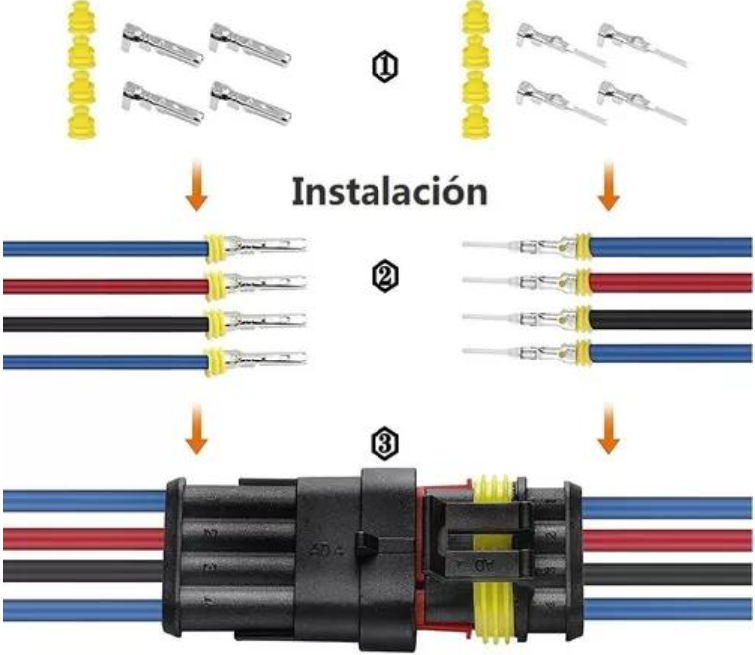
\includegraphics[width=0.7\textwidth]{figura40.png}
    \caption{Proceso de ponchado de cables.}
    \label{fig:ponchado}
\end{figure}

\subsubsection{Recubrimiento}
Ejemplo de cómo se ve el trenzado en la Fig. \ref{fig:trenzado}.

\begin{figure}[H]
    \centering
    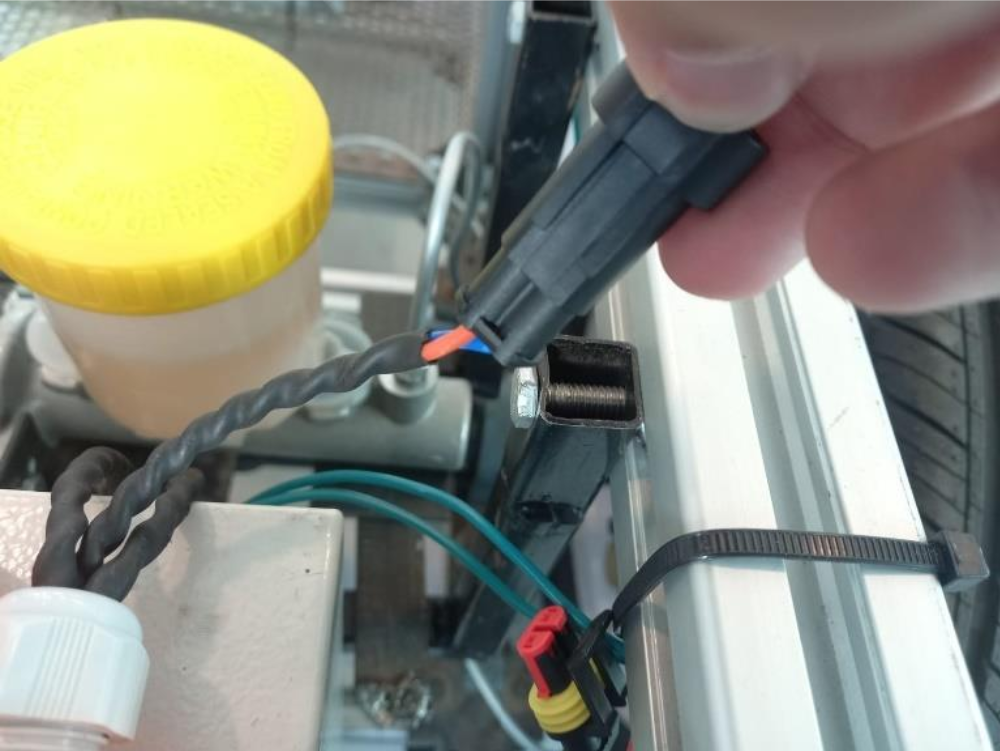
\includegraphics[width=0.7\textwidth]{figura41.png}
    \caption{Ejemplo de cómo se ve el trenzado de los cables CAN.}
    \label{fig:trenzado}
\end{figure}

\subsubsection{Especificaciones adicionales}
Un ejemplo de etiquetas en los cables es mostrado en la Fig. \ref{fig:etiquetado}.

\begin{figure}[H]
    \centering
    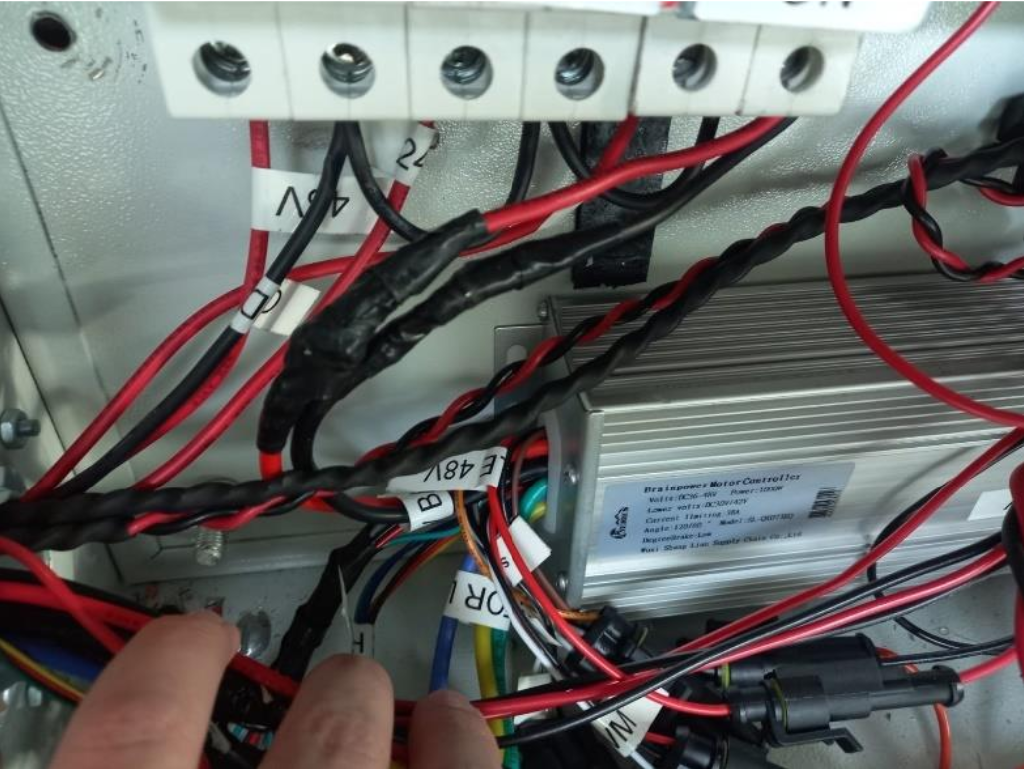
\includegraphics[width=0.7\textwidth]{figura42.png}
    \caption{Ejemplo del etiquetado de algunos de los cables dentro del tablero de control.}
    \label{fig:etiquetado}
\end{figure}

\section{Baterías}
\label{sec:baterias}

\subsection*{¿Cómo cargar las baterías?}
\addcontentsline{toc}{subsection}{¿Cómo cargar las baterías?}
Conectar las baterías en paralelo.
Dependiendo del número de baterías, seleccionar la corriente.

\begin{table}[H]
\centering
\caption{Configuraciones de carga}
\label{tab:conf_carga}
\begin{tabular}{ccccc}
\toprule
\textbf{Número} & \textbf{Corriente (Amps)} & \textbf{Tiempo máximo} & \textbf{Volt. inicial (V)} & \textbf{Volt. final (V)} \\
\midrule
1 & 2 & 5 horas o más &  &  \\
2 & 2 & 5 horas o más &  &  \\
3 & 10 & 9 horas & 12.3 & 12.8 \\
4 & 10 & 9 horas o más &  &  \\
4 & 40 & 5 horas & 12 & 12.5 \\
5 & 40 & 5 horas &  &  \\
\bottomrule
\end{tabular}
\end{table}

\subsection*{Consideraciones importantes:}
\addcontentsline{toc}{subsection}{Consideraciones importantes:}
Se está usando un cargador Schumacher SE4022, no obstante, la perilla del tiempo no funciona correctamente.

\subsection*{Precauciones:}
\addcontentsline{toc}{subsection}{Precauciones:}
Se debe de tener en constante supervisión a las baterías mientras se cargan.

\section{Seguridad del Vehículo}
\label{sec:seguridad}
\subsection{Botón paro de emergencia}
El diseño de la PCB se muestra en la Fig. \ref{fig:pcb_paro} y puedes encontrar el archivo Gerber en la \href{#}{siguiente carpeta}.

\begin{figure}[H]
    \centering
    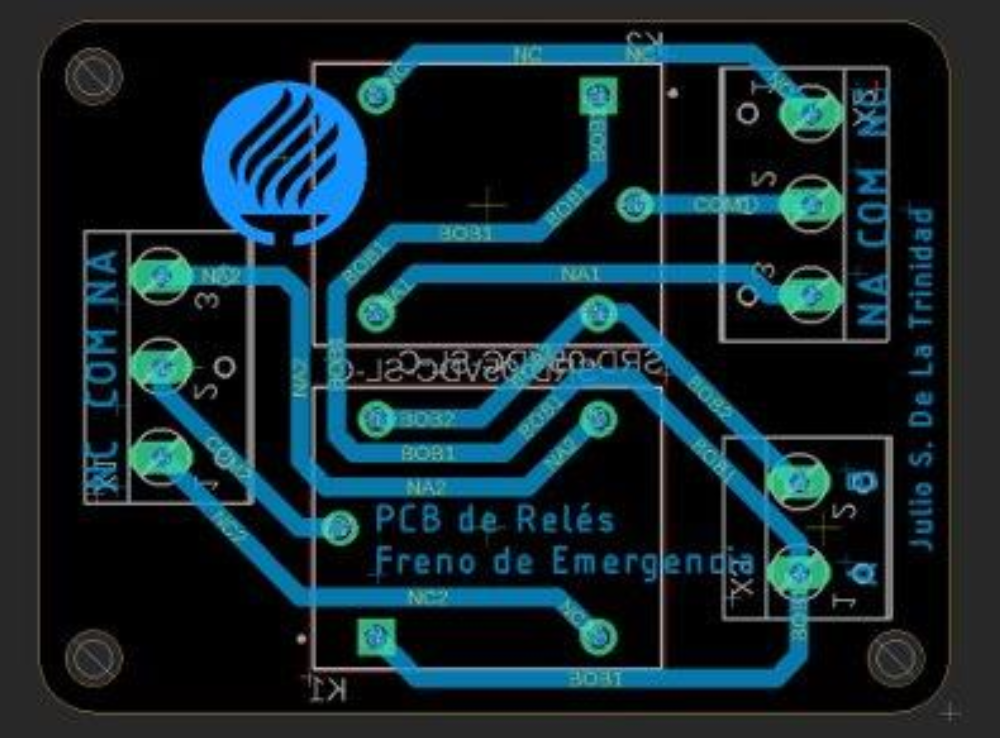
\includegraphics[width=0.6\textwidth]{figura43.png}
    \caption{Diseño de la PCB del paro de emergencia.}
    \label{fig:pcb_paro}
\end{figure}

Lista de componentes en la Tabla \ref{tab:comp_paro}.

\begin{table}[H]
\centering
\caption{Lista de componentes para la PCB del paro de emergencia.}
\label{tab:comp_paro}
\begin{tabular}{cl}
\toprule
\textbf{CANTIDAD} & \textbf{ELEMENTO} \\
\midrule
1 & Clema 2 Posiciones \\
2 & Clema 3 Posiciones \\
2 & Relés Sonoff 5 V \\
\bottomrule
\end{tabular}
\end{table}

\section{Sistema de navegación}
\label{sec:navegacion}
Se implementará durante el semestre FJ23.

\end{document}